\clearpage
\section{Methods}\label{section::Methods}

This chapter presents our complete method for accurate crowd counting on railway platforms. We propose a detect–track–count pipeline that combines YOLOv11m head detection, EfficientNet-B0-based ReID feature extraction, and three Kalman state-space configurations within DeepSORT for robust multi-object tracking. Our key innovation is the Phys-6D physics-constrained tracker that leverages camera geometry and scene priors to stabilize identity consistency and achieve superior counting accuracy. The complete system architecture, implementation details, and algorithmic specifications are provided in this chapter, with experimental validation and comparative analysis presented in \textbf{Chapter~5}.



\subsection{Proposed Method (Our Method)}

We tackle platform crowd counting with a detect–track–count pipeline tailored to station-arrival videos with dense occlusions and strong perspective effects. (\textbf{Fig.}~\ref{fig:OurMOTSystemArchitecture}) shows the overall multi-object tracking system architecture.
\begin{figure}[H]
    \centering
    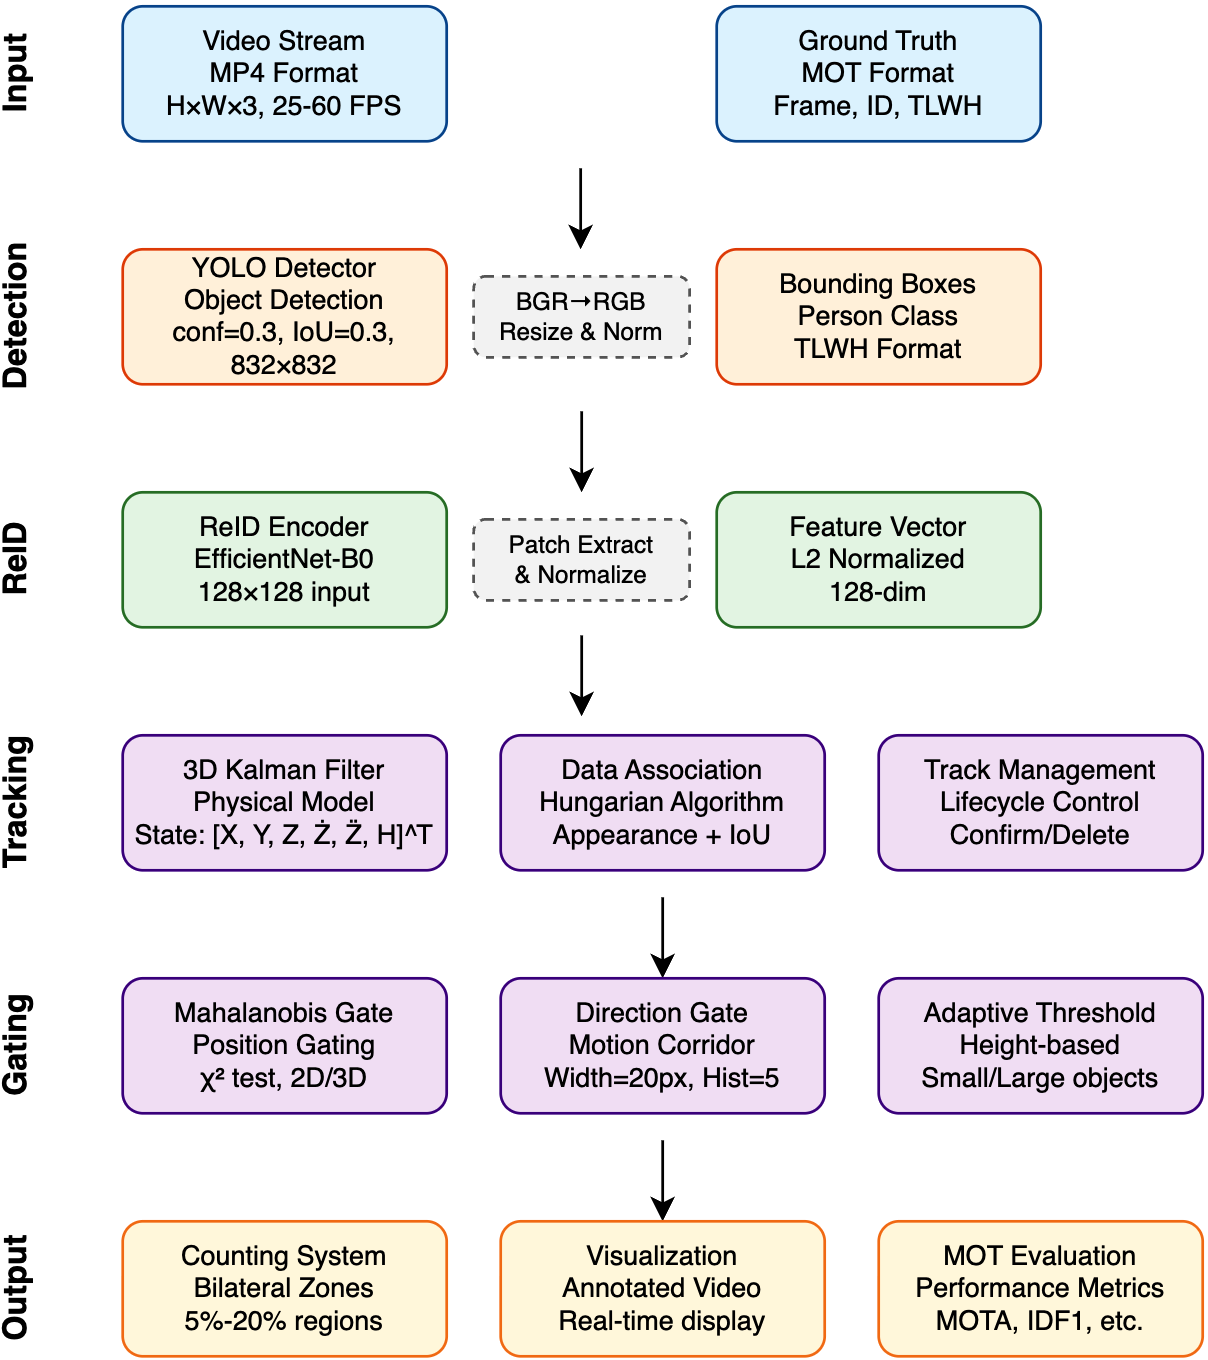
\includegraphics[width=0.8\textwidth]{pictures/OurMulti-ObjectTrackingSystemArchitecture.png}
\caption{Overall Multi-object Tracking System Architecture. The system integrates YOLOv11-based object detection, EfficientNet-B0 ReID feature extraction, and a 3D physical Kalman filter for robust pedestrian tracking. The pipeline consists of five modules: (1) Input, which includes video streams and ground-truth annotations in MOT format; (2) Detection, where YOLOv11 detects pedestrian bounding boxes (TLWH format); (3) ReID, which extracts 128-dimensional L2-normalized feature vectors using an EfficientNet-B0 encoder; (4) Tracking and Gating, which performs data association via a Hungarian algorithm combining appearance and IoU metrics, managed by a 3D Kalman filter with state variables ${[X,\ Y,\ Z,\ \dot{Z},\ \ddot{Z},\ H]}$ and multiple gating strategies including Mahalanobis distance, directional motion corridors, and adaptive thresholds; and (5) Output, which provides bilateral-zone counting, annotated visualization, and MOTChallenge performance evaluation (MOTA, IDF1, etc.). This modular architecture ensures accurate, stable, and interpretable tracking across video sequences.}
    \label{fig:OurMOTSystemArchitecture}
\end{figure}

\subsection{Scene and Imaging Model}
We model a forward-facing camera rigidly mounted near the train head, with the optical axis aligned with the track tangent. Pedestrians on the platform stand at lateral distance $X$ from the track centerline and have 3D vertical coordinate $Y$ (both approximately constant over time in the camera frame). Let $(u,v)$ be pixel coordinates with intrinsics $(f,c_x,c_y)$, where $f$ is the focal length (in pixels), $c_x$ is the principal point x-coordinate, and $c_y$ is the principal point y-coordinate. Denote by $Z(t)$ the depth coordinate along the track direction from camera to a target head. During arrival, motion is captured by
\begin{equation}
Z(t)=Z_0+\dot{Z}_0 t + \tfrac{1}{2}\ddot{Z}\,t^{2}, \quad \ddot{Z}<0.
\end{equation}
Under a pinhole model the projection obeys
\begin{equation}
u(t)=c_x+f\tfrac{X}{Z(t)},\quad v(t)=c_y+f\tfrac{Y}{Z(t)},\quad h_{\text{px}}(t)=f\tfrac{H(t)}{Z(t)},
\end{equation}
where $H(t)$ represents the physical head height above the platform surface, and $Z(t)$ is the depth coordinate in the camera coordinate system (with $Z_t$ pointing along the track towards the platform). This provides a stable mapping between apparent size and depth. This scene model underpins the Phys-6D tracker by explicitly coupling pixel height $h_{\text{px},t}$ and depth $Z_t$, and guides counting-band placement near image borders where perspective magnification and occlusions are prominent. Camera intrinsics used in experiments are reported with the calibration results in Chapter~5.

\textbf{Figure}~\ref{fig:3TrackingTrackGraph} illustrates the 2D planar trajectory visualization of human head bounding box centers from three video sequences, generated from MOT-format ground truth annotations. This visualization demonstrates the typical movement patterns and spatial distribution of pedestrian trajectories in our railway platform scenarios.

\begin{figure}[H]
    \centering
    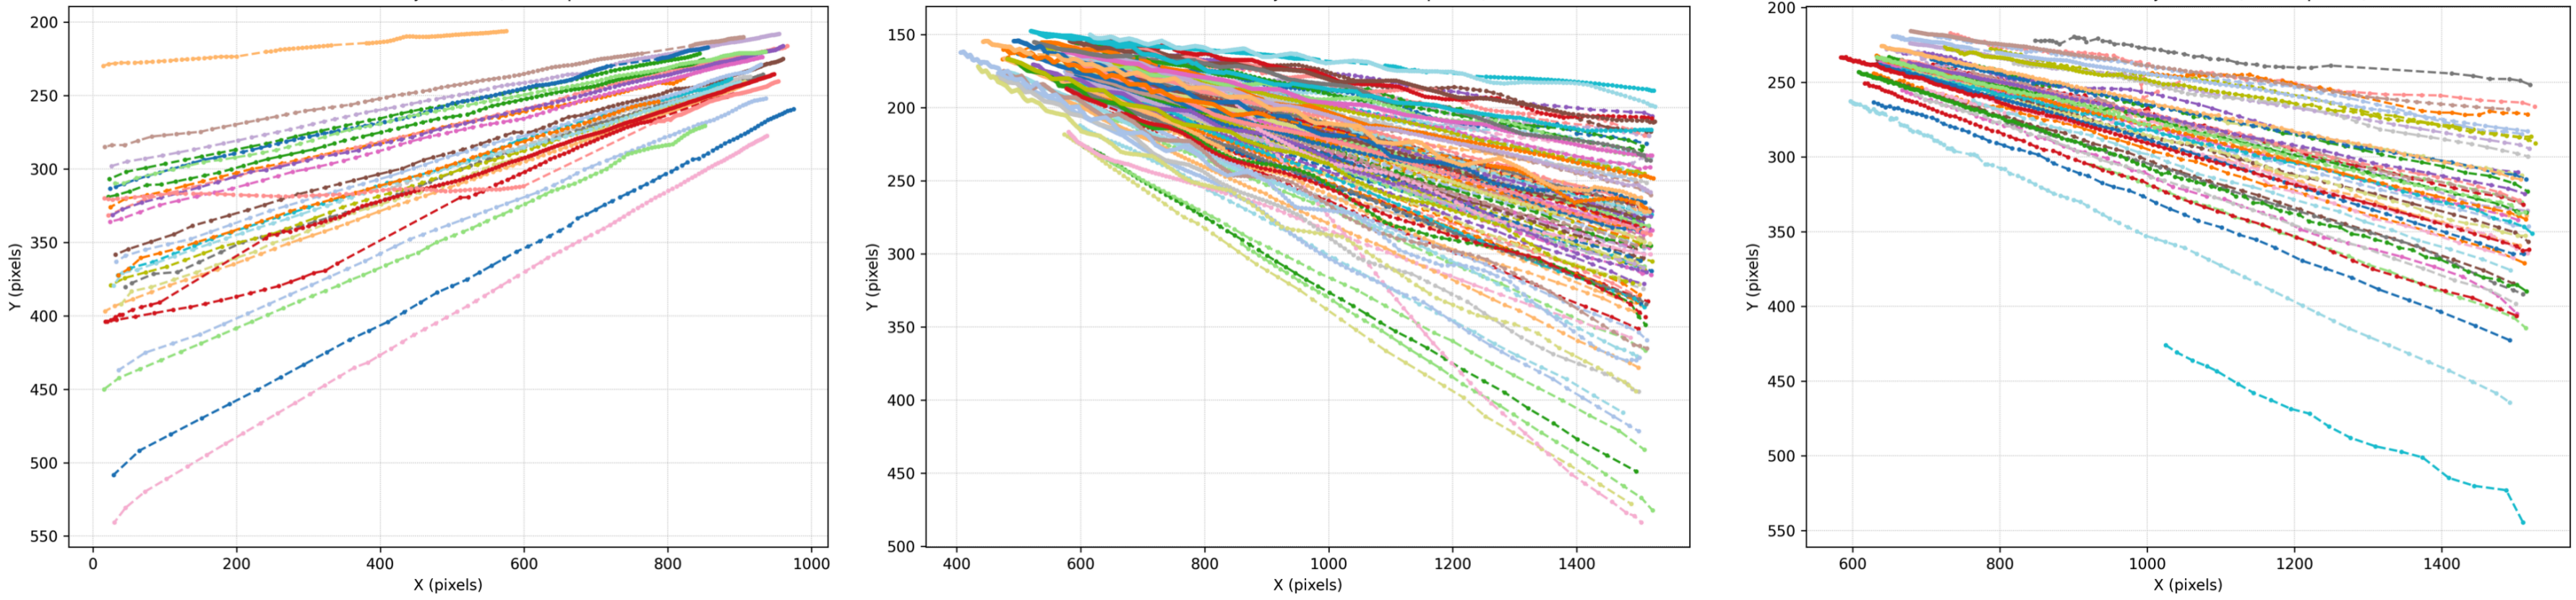
\includegraphics[width=0.95\textwidth]{pictures/3 Tracking Track Graph.png}
    \caption{2D planar trajectory visualization of human head bounding box centers from three video sequences, generated from MOT-format ground truth annotations.}
    \label{fig:3TrackingTrackGraph}
\end{figure}


\subsection{Implementation Details}
We provide complete implementation specifications for reproducibility:

\textbf{Detector Configuration:} YOLOv11m with two-stage transfer learning: (1) pre-train on CrowdHuman dataset; (2) fine-tune on railway/platform head images with the first 10 backbone layers frozen. Training uses SGD optimizer (lr=1e-2, weight decay=5e-4), cosine annealing scheduler, and mixed precision. Inference thresholds: confidence=0.5, IoU=0.7, input size=640×640.

\textbf{ReID Configuration:} EfficientNet-B0 backbone with input preprocessing: direct resizing to target size (128x128), horizontal flip augmentation, and color jitter. Training uses triplet loss with margin α=0.5, Adam optimizer (lr=1e-4), StepLR scheduler (step\_size=10, gamma=0.5).

\textbf{Tracking Configuration:} DeepSORT with three Kalman state-space configurations. Association uses linear combination of Mahalanobis distance (motion) and cosine distance (appearance) with weight λ=0.5. Cascaded matching prioritizes recently observed tracks. Gating thresholds: CV-8D uses standard DeepSORT thresholds; CA-12D uses stricter thresholds due to higher dimensionality;Phys-6D uses geometry-aware thresholds based on depth constraints.

\textbf{Counting Configuration:} Virtual counting bands with Start=0.05, End=0.20 (relative to image width), persistence threshold N=2 frames. Per-ID de-duplication and end-of-video compensation are applied. Final count uses maximum of left/right counts to avoid non-platform bias.

\textbf{System Integration:} All components run on GPU with real-time processing capability. The complete pipeline processes video frames sequentially: detection → ReID feature extraction → Kalman prediction → data association → track update → counting logic.

\subsection{YOLOv11 Model}

In our method, YOLOv11m is used specifically for head detection to reduce occlusion-induced misses on full bodies and to stabilize localization for small targets. We adopt transfer learning and fine-tuning to specialize for platform heads (details summarized below and results in Chapter~5), while retaining the architectural advantages of YOLOv11 for real-time deployment.

In 2015, Redmon et al. introduced the YOLO algorithm, a landmark in object detection \cite{76_redmon2016lookonceunifiedrealtime}. As its name suggests, YOLO detects objects and their locations in a single pass over the image by formulating detection as a regression problem, in contrast to traditional two-stage pipelines. As illustrated in \textbf{Fig.}~\ref{fig:yolosystem-cn} and \textbf{Fig.}~\ref{fig:yoloarchitecture-cn}, a single convolutional neural network (CNN) jointly predicts bounding boxes and class probabilities across the entire image \cite{77_Du_article}, simplifying the detection process compared to more complex traditional methods. Recent studies have demonstrated the computational efficiency advantages of YOLO-based approaches in edge computing scenarios, where single-stage detection models can reduce resource usage by nearly 50\% compared to multiple specialized networks \cite{s23136138}.
\begin{figure}[H]
    \centering
    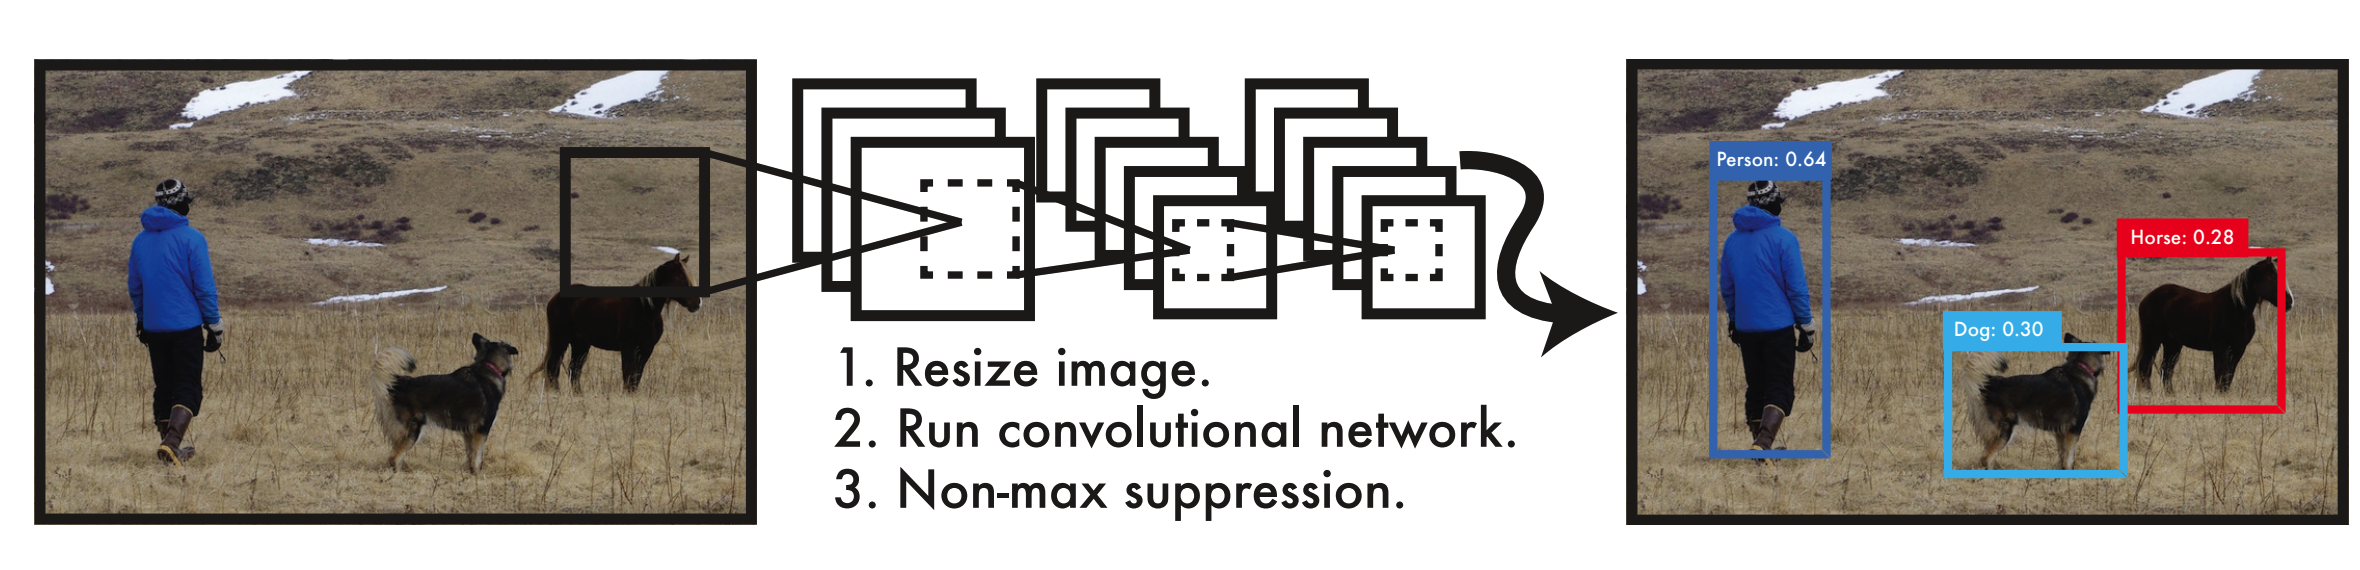
\includegraphics[width=0.8\textwidth]{pictures/The YOLO Detection System.png}
    \caption{YOLOv1 Detection System \cite{76_redmon2016lookonceunifiedrealtime}}
    \label{fig:yolosystem-cn}
\end{figure}
\begin{figure}[H]
    \centering
    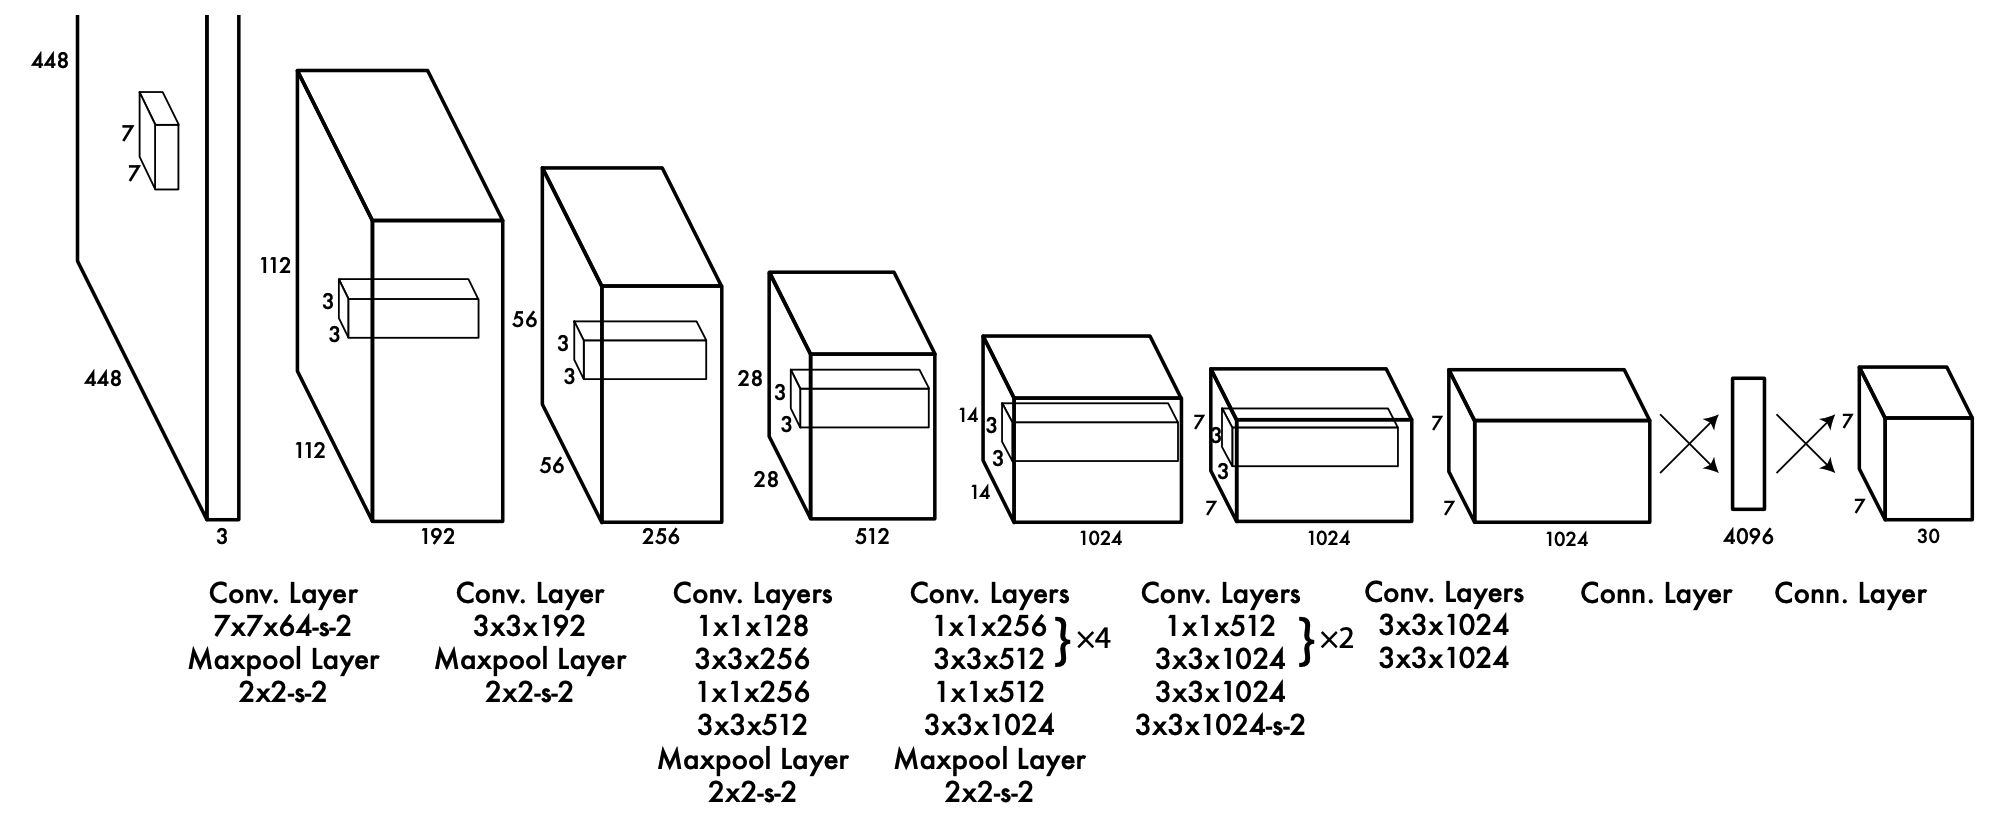
\includegraphics[width=0.8\textwidth]{pictures/The YOLO Architecture.png}
    \caption{YOLOv1 Architecture \cite{76_redmon2016lookonceunifiedrealtime}}
    \label{fig:yoloarchitecture-cn}
\end{figure}

YOLOv11 represents a significant step forward in the YOLO family, announced at the YOLOVision 2024 (YV24) conference. It refines network design and training strategies to further improve detection accuracy and speed \cite{74_yolo11_Jocher_Ultralytics_YOLO_2023}. As noted in Related Work, using full-body cues for detection degrades substantially in crowded scenes due to heavy occlusions, whereas head cues are more discriminative and less occluded yet remain underexplored. In high-density settings, frequent and severe occlusions hinder full-body recognition, while heads, being at the upper body and less occluded with more stable shape cues, are easier to localize. Head sizes also vary less with pose, reducing both false positives and false negatives. Accordingly, we detect heads with YOLOv11 as the basis for counting.

As shown in \textbf{Fig.}~\ref{fig:benchmarkingyolo11}, YOLOv11 introduces notable architectural and training enhancements that push the boundary of accuracy, speed, and efficiency \cite{75_khanam2024yolov11overviewkeyarchitectural}.
\begin{figure}[H]
    \centering
    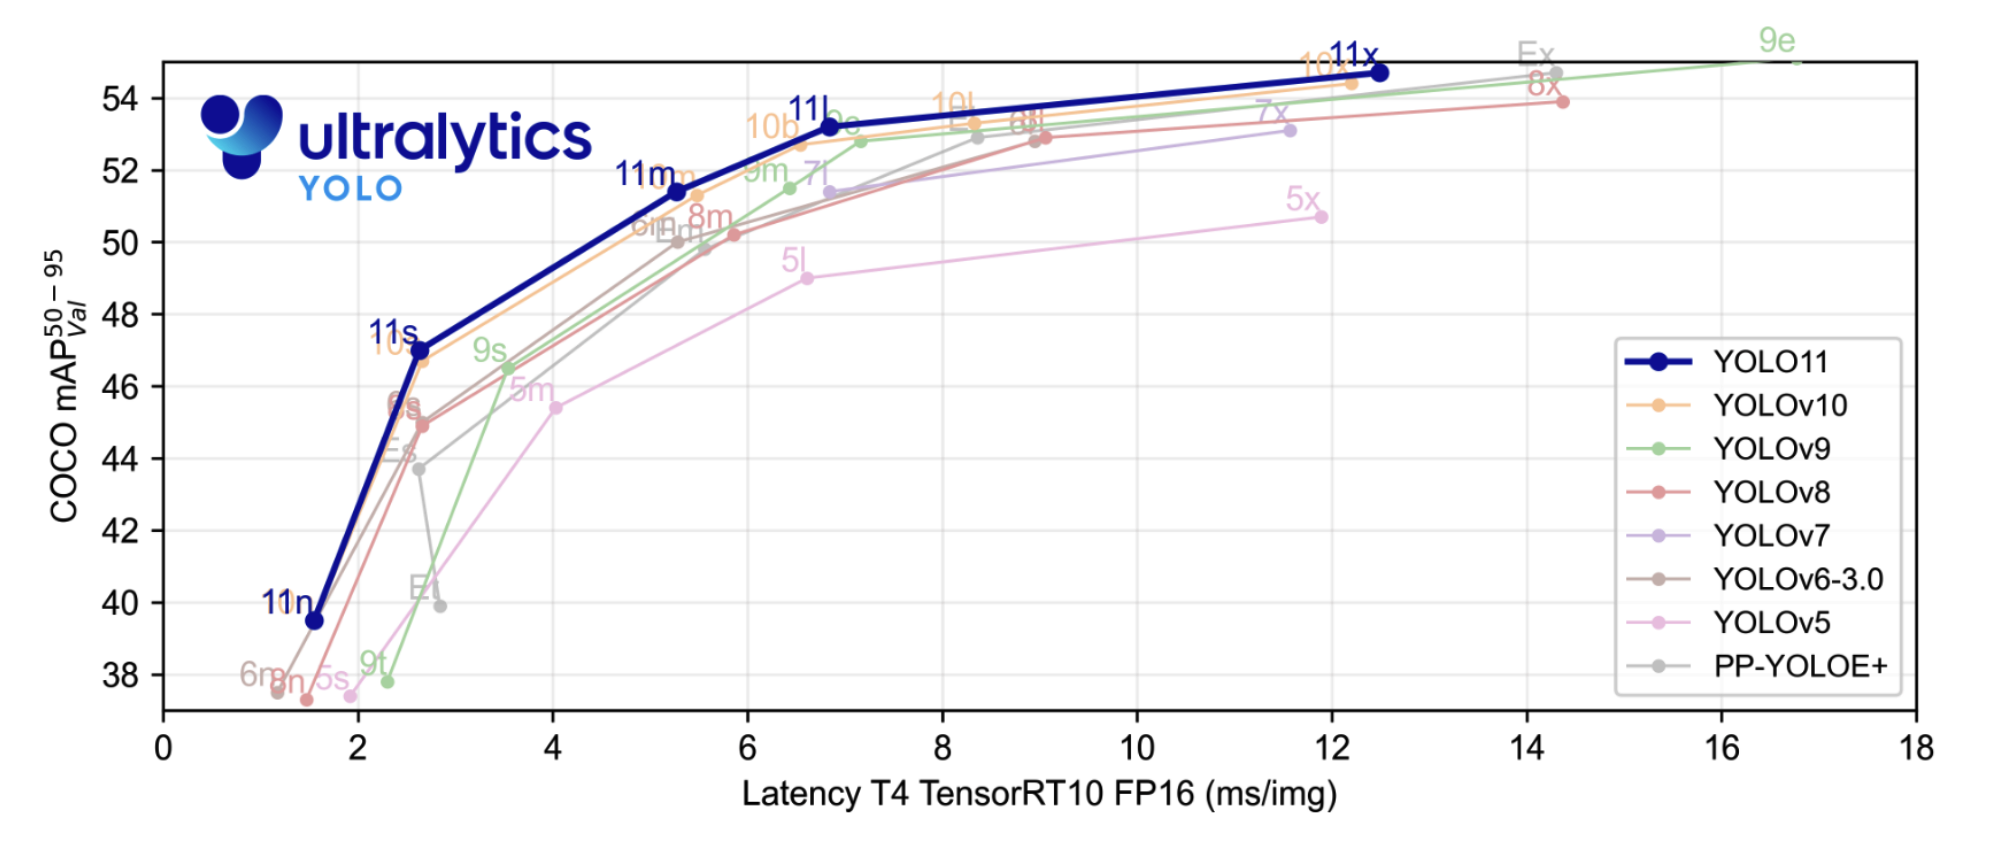
\includegraphics[width=0.6\textwidth]{pictures/BenchmarkingYOLOv11AgainstPrevious Versions.png}
    \caption{Benchmarking YOLOv11 Against Previous Versions\cite{74_yolo11_Jocher_Ultralytics_YOLO_2023}}
    \label{fig:benchmarkingyolo11}
\end{figure}




\subsection{Key Architectural Components of YOLOv11}
The YOLOv11 architecture comprises three fundamental components (\textbf{Fig.}~\ref{fig:yolo11architecture-cn}). First, the backbone serves as the primary feature extractor, transforming raw images into multi-scale feature maps via CNNs. Second, the neck acts as an intermediate aggregation stage, enhancing and fusing features across scales. Third, the head produces the final predictions for localization and classification \cite{75_khanam2024yolov11overviewkeyarchitectural}.

\begin{figure}[H]
    \centering
    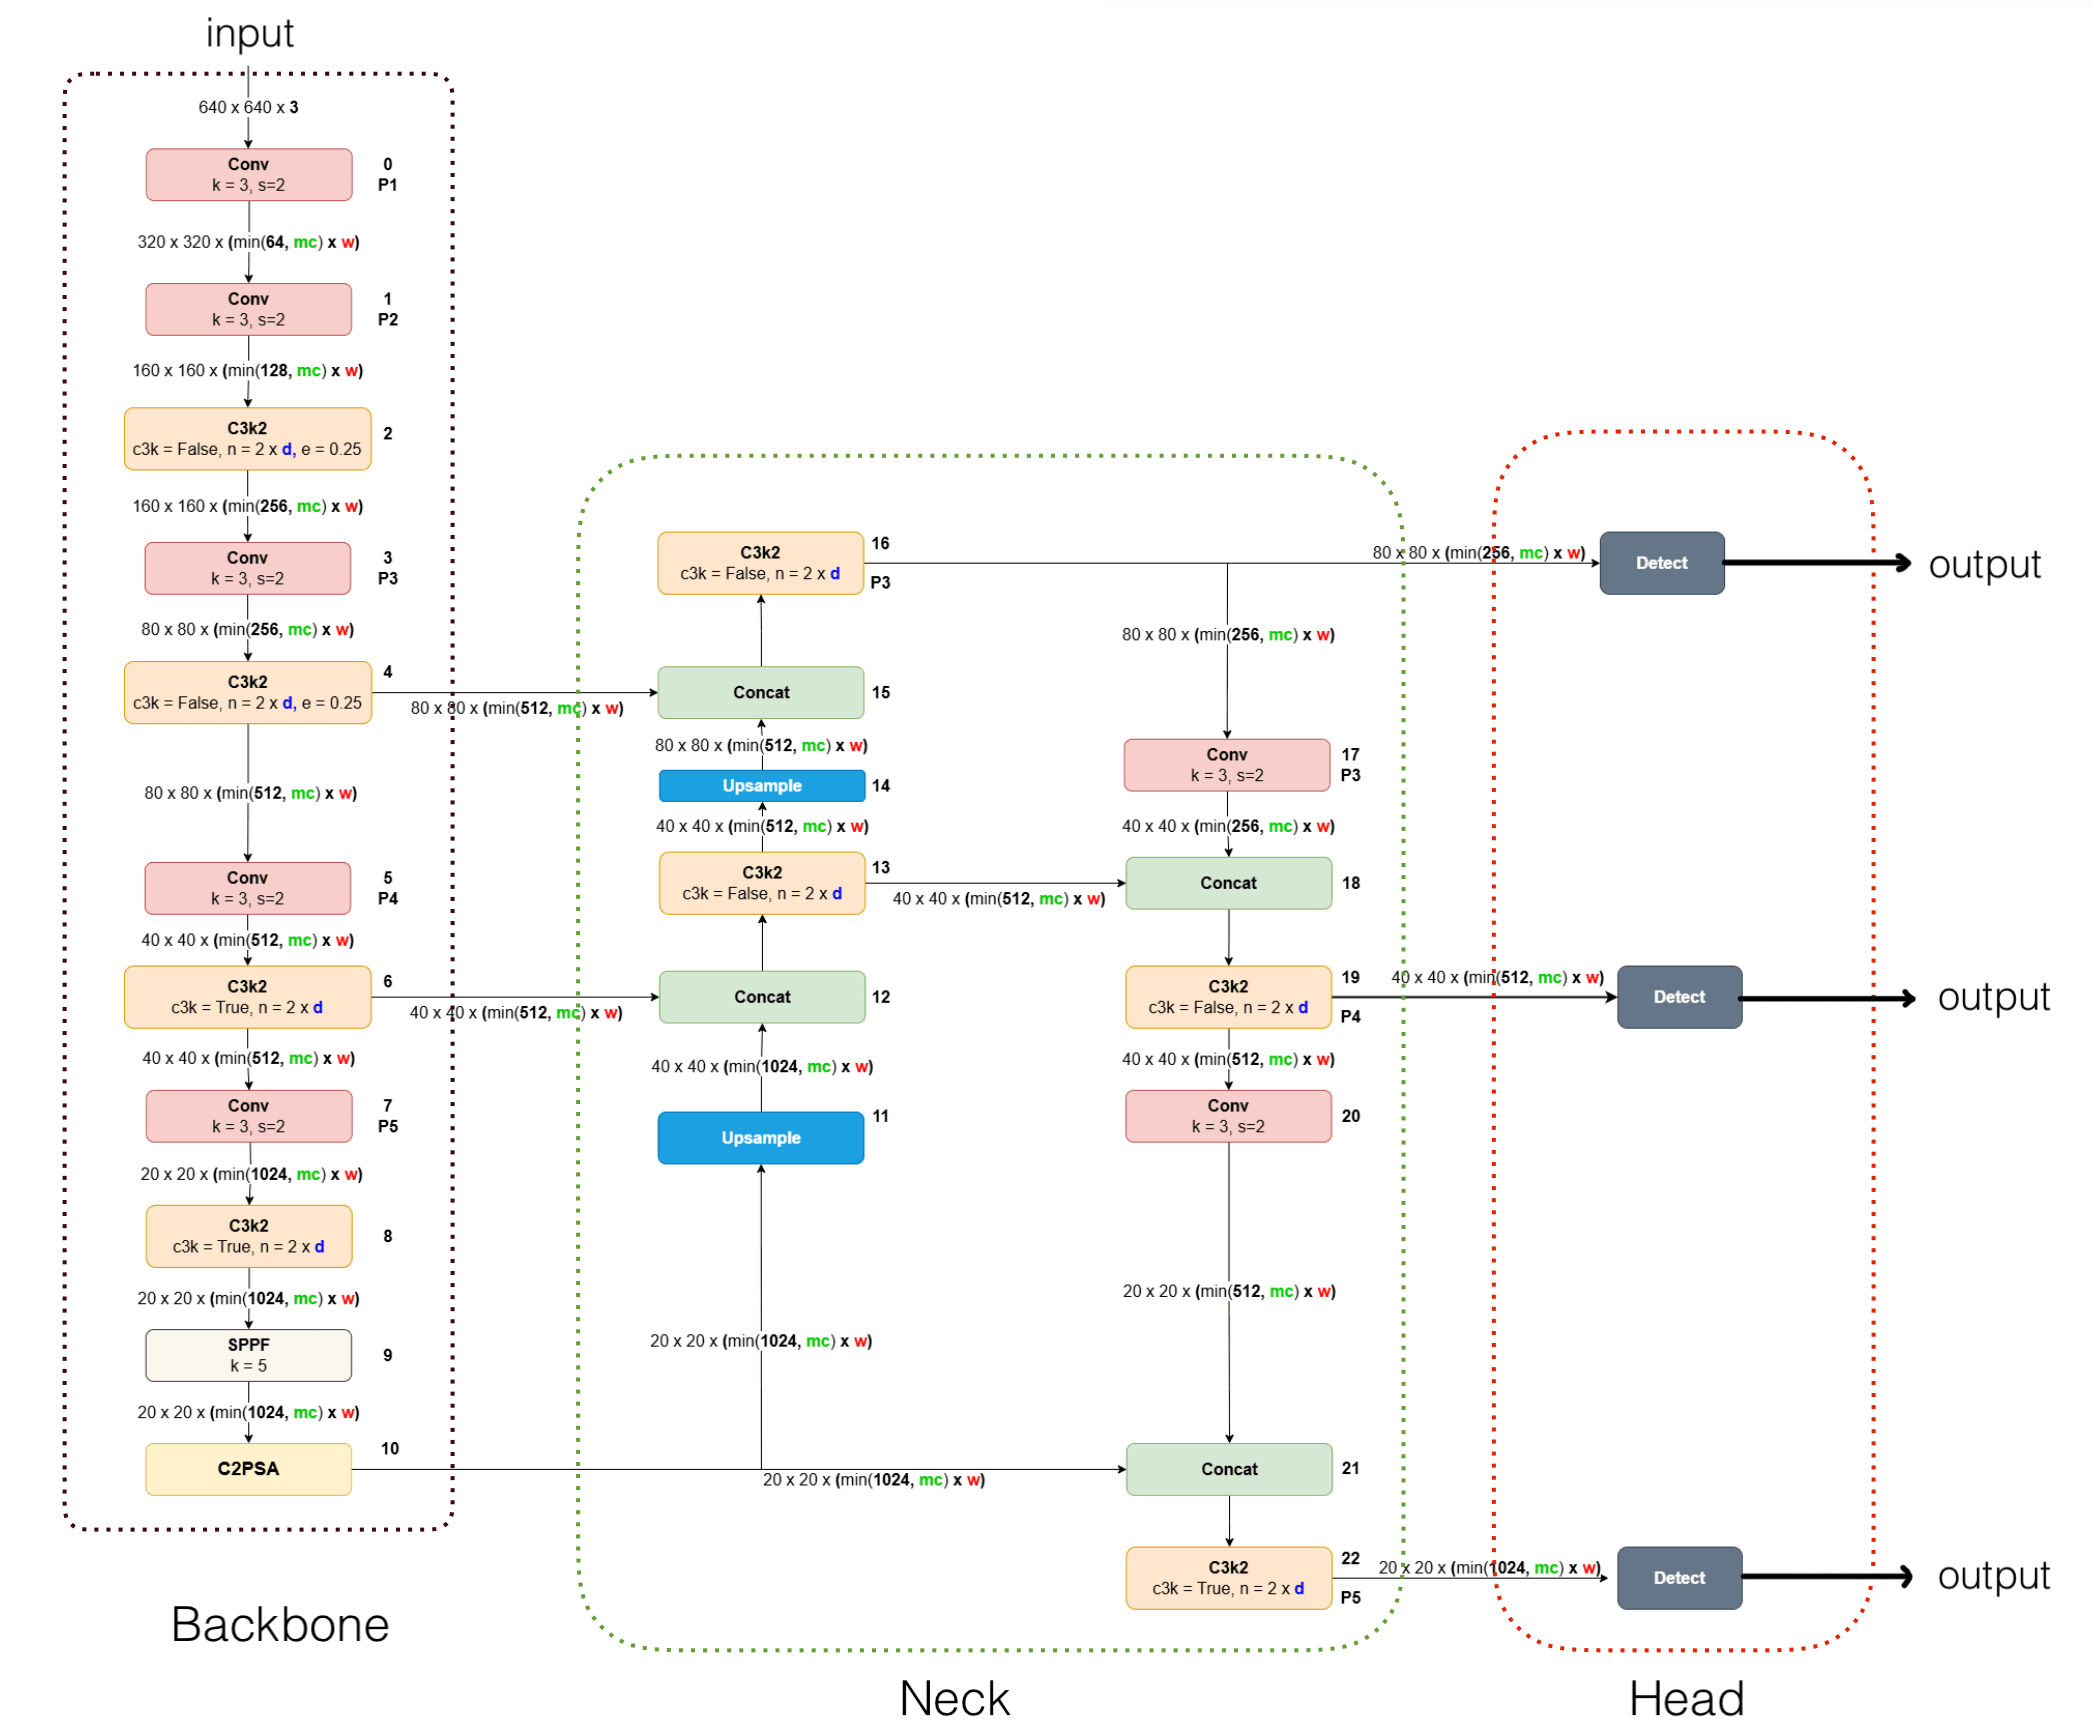
\includegraphics[width=0.92\textwidth]{pictures/Yolo11architecture.png}
    \caption{YOLOv11 Architecture\cite{80_ghosh_yolo11_2024}}
    \label{fig:yolo11architecture-cn}
\end{figure}

YOLOv11 introduces significant architectural and training enhancements that push the boundaries of accuracy, speed and efficiency. As shown in \textbf{Fig.}~\ref{fig:Keyarchite-cn}, the key architectural components of YOLOv11 are illustrated.
\begin{figure}[H]
    \centering
    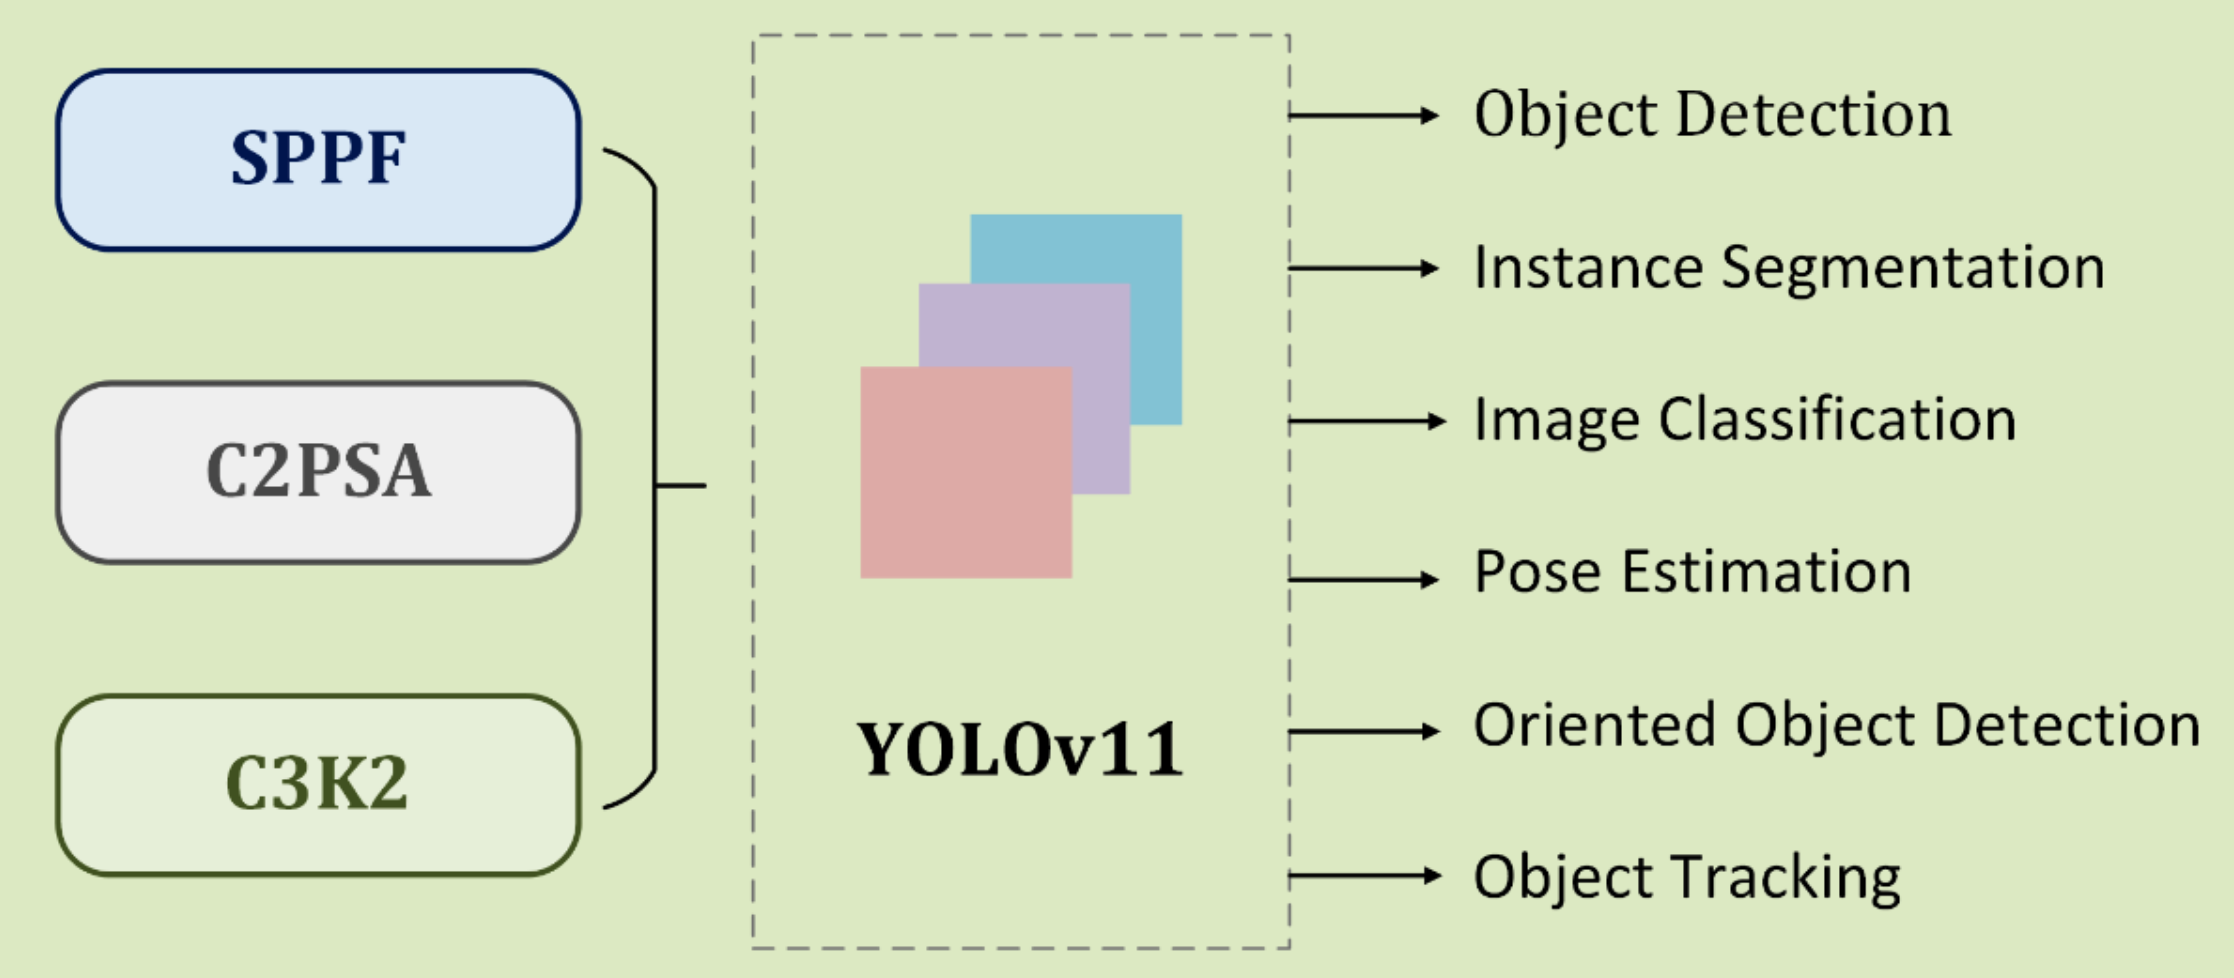
\includegraphics[width=0.7\linewidth]{pictures/key architectural modules in YOLO11.png}
    \caption{Key Architectural Modules in YOLOv11 \cite{80_ghosh_yolo11_2024}}
    \label{fig:Keyarchite-cn}
\end{figure}

\subsubsection{Backbone Network}
The backbone extracts features at multiple scales by stacking convolutional layers and specialized blocks to produce feature maps at varying resolutions. Initial convolutional layers downsample the input, progressively reducing spatial dimensions while increasing channel depth.

\paragraph{SPPF and C2PSA}
YOLOv11 retains the Spatial Pyramid Pooling - Fast (SPPF) block and introduces the Cross Stage Partial with Spatial Attention (C2PSA) block \cite{80_ghosh_yolo11_2024}. As shown in \textbf{Fig.}~\ref{fig:C2PSA-cn}, C2PSA enhances spatial attention, enabling the model to focus more effectively on salient regions. By pooling spatial features, C2PSA strengthens localization of objects at different sizes and positions.
\begin{figure}[H]
    \centering
    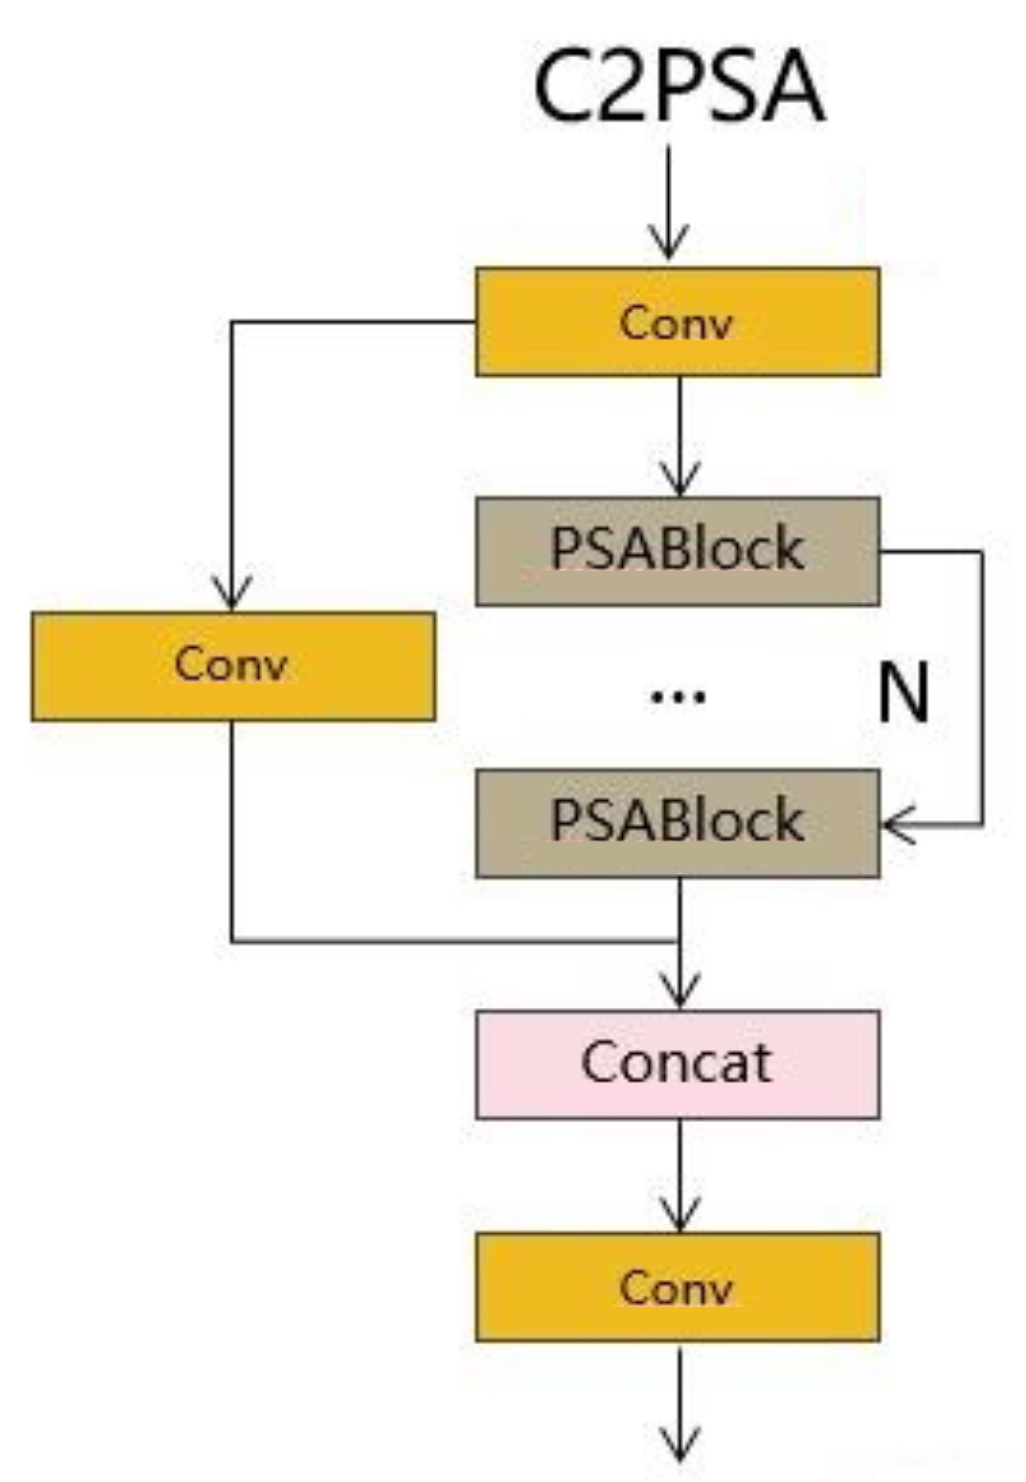
\includegraphics[width=0.25\linewidth]{pictures/C2PSA.png}
    \caption{YOLOv11 C2PSA Module \cite{80_ghosh_yolo11_2024}}
    \label{fig:C2PSA-cn}
\end{figure}

\subsubsection{Neck Network}
The neck bridges backbone and head, aggregating features from multiple scales for downstream prediction.

\paragraph{C3K2 block}
YOLOv11 replaces the neck's C2f blocks with C3k2 blocks, a more computationally efficient variant of the CSP (Cross Stage Partial) bottleneck. As shown in \textbf{Fig.}~\ref{fig:C3K2-cn}, it uses two smaller convolutions instead of a single large convolution (as in YOLOv8 \cite{81_noauthor_what_2024}). The "k2" indicates smaller kernel sizes, improving speed while maintaining performance \cite{75_khanam2024yolov11overviewkeyarchitectural}.
\begin{figure}[H]
    \centering
    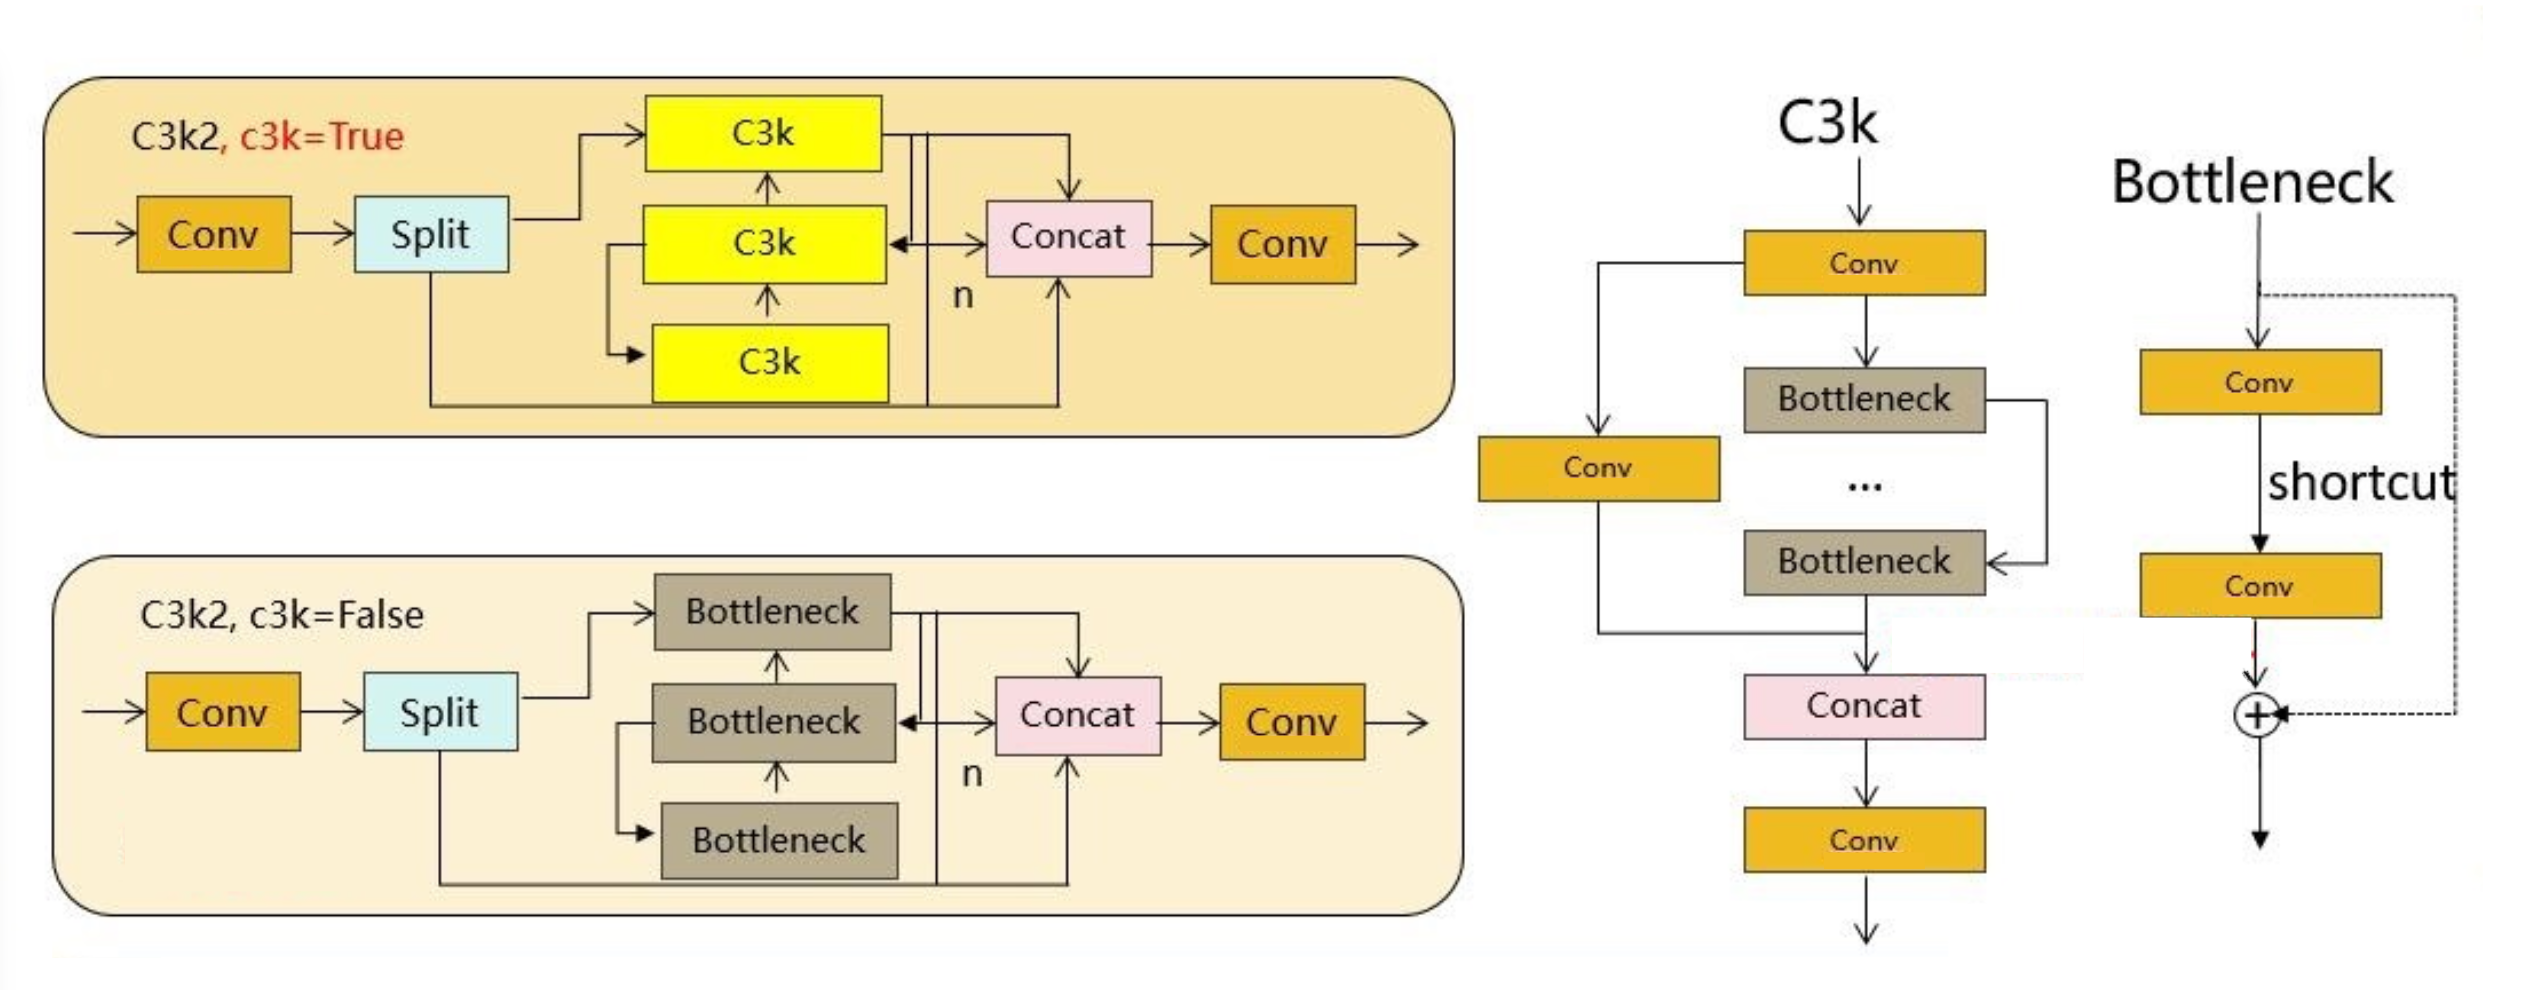
\includegraphics[width=0.8\linewidth]{pictures/C3K2.png}
    \caption{C3K2 Module\cite{83_ultralytics_yolo11_2025}}
    \label{fig:C3K2-cn}
\end{figure}

Attention mechanism
An important addition in YOLOv11 is increased emphasis on spatial attention via C2PSA. This mechanism helps focus on key regions, yielding more accurate detection of small or partially occluded objects. This distinguishes YOLOv11 from YOLOv8, which lacks this specific attention module \cite{80_ghosh_yolo11_2024,75_khanam2024yolov11overviewkeyarchitectural}.

\subsubsection{Detection Head}
The head performs multi-scale predictions, outputting bounding-box parameters (center, width, height), class probabilities, and objectness scores. The input image is partitioned into grid cells, each responsible for objects whose centers fall within it.

\paragraph{C3k2 blocks}
YOLOv11 employs multiple C3k2 blocks within the head to process and refine features across different depths. Behavior varies with the parameter c3k:\\
    • If c3k = False, C3k2 behaves similarly to C2f with a standard bottleneck.\\
    • If c3k = True, the bottleneck is replaced with a C3 module for deeper, more expressive feature extraction.\\
Key properties of C3k2:\\
    • Faster processing via two smaller convolutions instead of a single large convolution.\\
    • Parameter efficiency as a more compact CSP bottleneck.\\
Additionally, the C3k module allows customizable kernel sizes for improved flexibility.

\paragraph{CBS blocks}
After C3k2 blocks, YOLOv11's head includes several CBS (Convolution–BatchNorm–SiLU) layers \cite{81_noauthor_what_2024}, which further refine features by extracting salient cues, stabilizing flow via batch normalization, and introducing nonlinearity through SiLU.

\paragraph{Final convolution and detection layers}  
Each detection branch ends with Conv2D layers that reduce features to the required outputs for bounding-box regression and classification. The final detection layer aggregates predictions:\\
    • Bounding-box coordinates for localization.\\  
    • Objectness scores.\\  
    • Class probabilities.\\

\subsection{DeepSORT}
We next introduce the DeepSORT multi-object tracker as used in our method. Our implementation extends the standard DeepSORT framework with several key modifications: (1) we replace the original CNN-based appearance extractor with EfficientNet-B0 for improved feature quality; (2) we introduce three different Kalman state-space configurations (CV-8D, CA-12D, and Phys-6D) instead of the standard constant-velocity model; and (3) we adapt the association thresholds and parameters for railway platform scenarios. Our tracker fuses appearance (EfficientNet-B0 embeddings) and motion (Kalman state-space models) with cascaded association to preserve identities under occlusions. Recent advances in multi-object tracking have demonstrated the effectiveness of combining local and global pose estimation for precise tracking of similar objects, particularly in scenarios with geometric ambiguities and occlusions \cite{pose_estimation_2022}. DeepSORT\cite{211}, an extension of SORT\cite{220}, combines deep appearance embeddings with motion information. The pipeline (\textbf{Fig.}~\ref{fig:DeepSORT-cn}) comprises deep appearance feature extraction, a Kalman filter, and data association.
\begin{figure}[H]
    \centering
    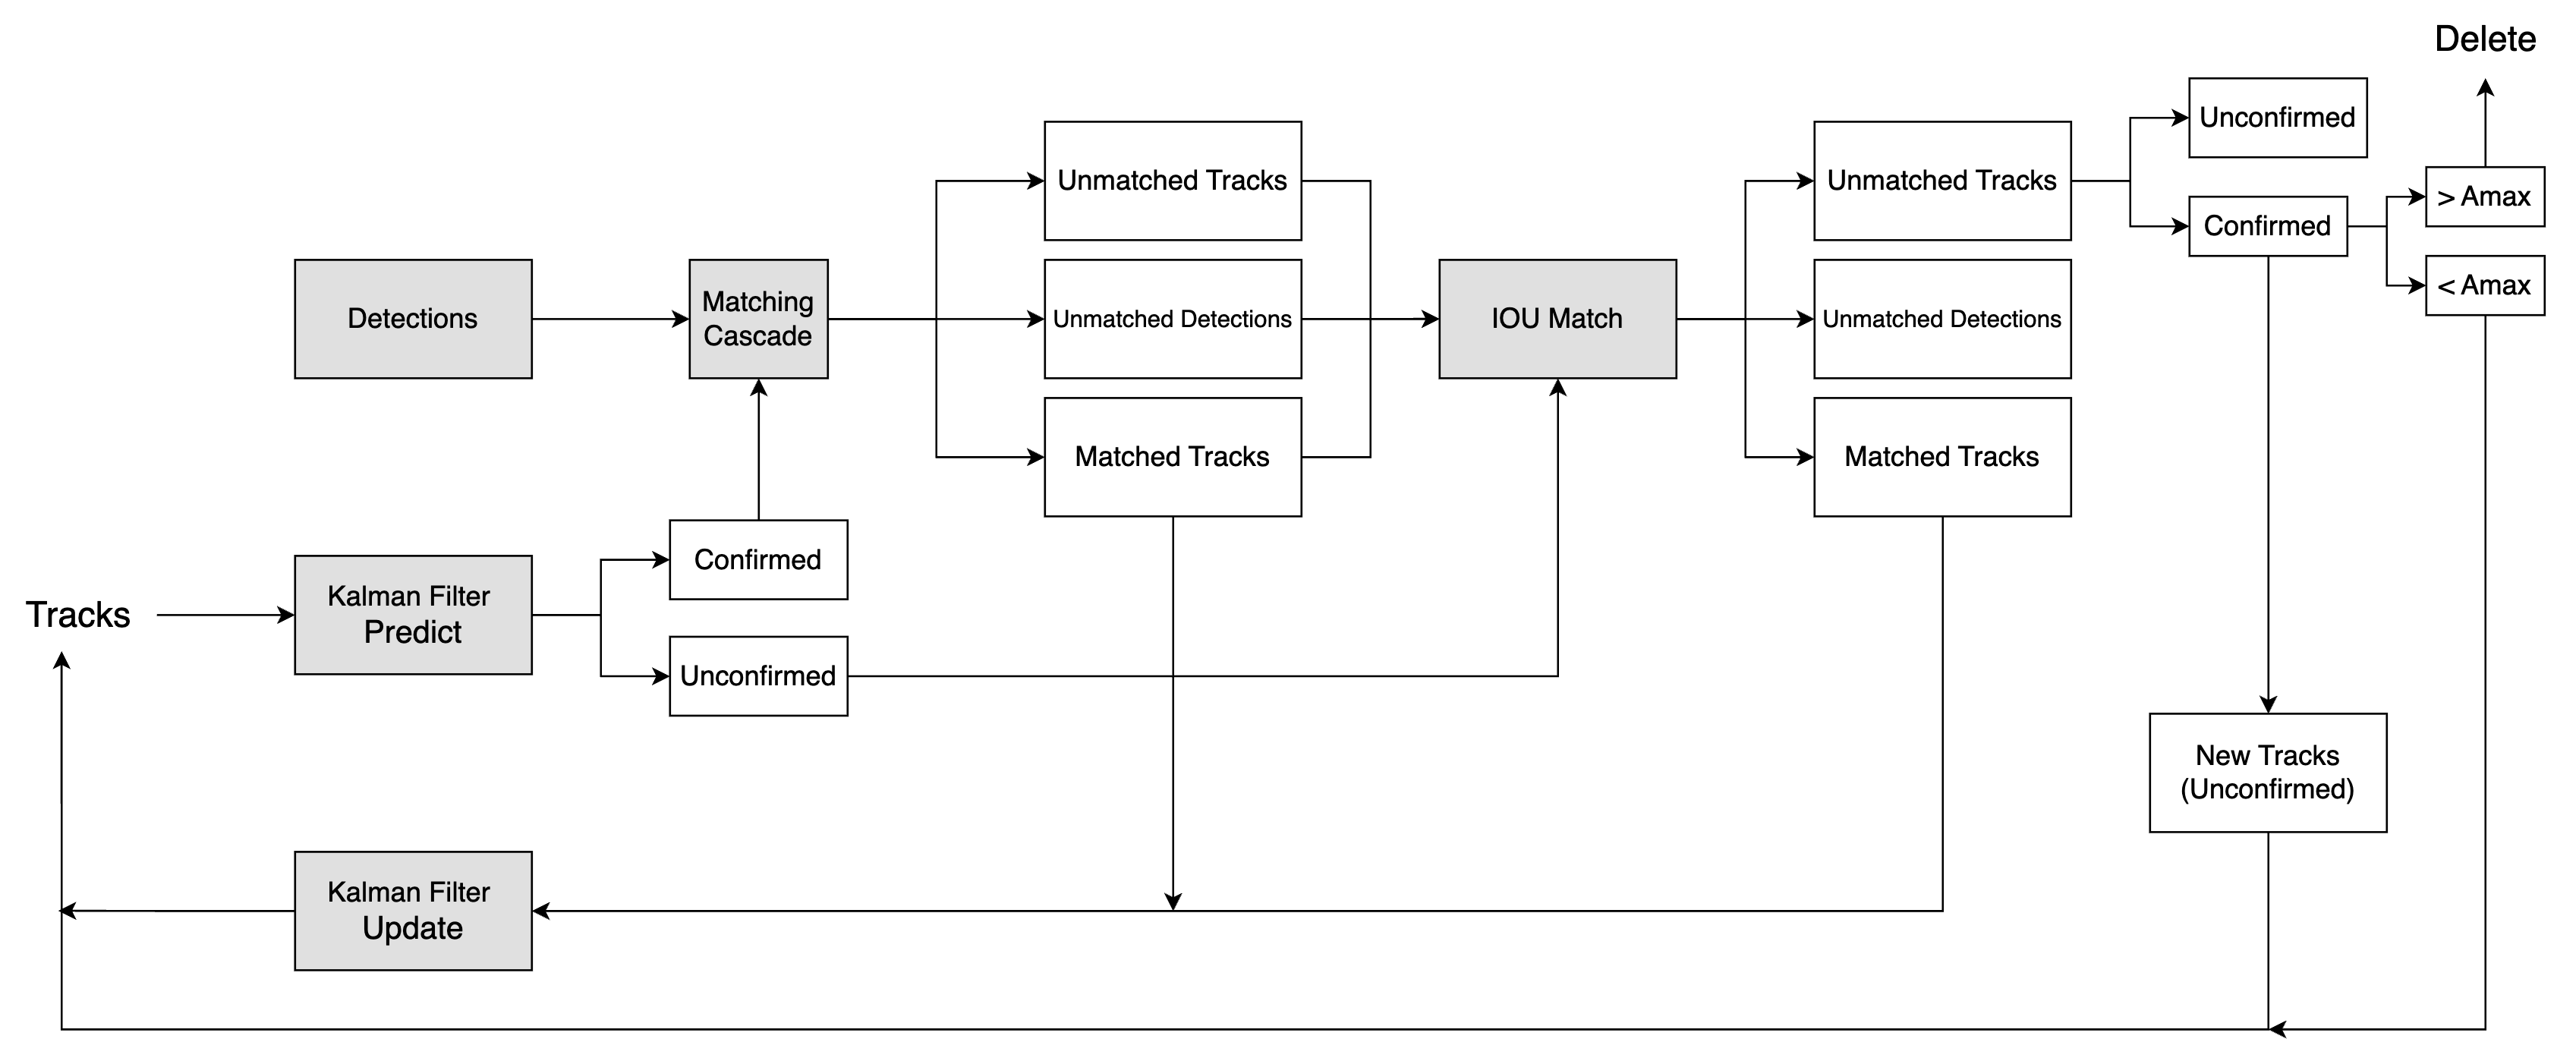
\includegraphics[width=0.99\textwidth]{pictures/DeepSORTAlgorithmStructure.png}
    \caption{DeepSORT architecture\cite{212}. The workflow can be summarized as follows:
    (1) Object detection: a high-performance detector identifies targets in each frame and outputs bounding boxes with confidences \cite{174}.
    (2) Motion prediction: a Kalman filter predicts current positions and motion states for existing tracks \cite{174}.
    (3) Feature extraction: deep appearance embeddings are computed for detections via a ReID model \cite{179}.
    (4) Data association: detections are matched to predicted tracks using a cost that combines motion (Mahalanobis distance) and appearance (cosine distance), solved with the Hungarian algorithm; a cascaded strategy further improves matching \cite{104}.
    (5) Track update and management: matched tracks are updated; unmatched detections initialize new tracks; long-unmatched tracks are terminated.}
    \label{fig:DeepSORT-cn}
\end{figure}



\subsection{DeepSORT Core Modules}

\subsubsection{Object Detector}
In our system, tracking performance depends critically on the head detector; we adopt YOLOv11m as detailed above. For completeness, typical detectors include:\\
• YOLO family: widely adopted for its real-time performance and accuracy (e.g., YOLOv5/YOLOv7), and in our case YOLOv11.\\
• Faster R-CNN: representative two-stage detector used in early variants.\\
• SSD: one-stage detector also used in DeepSORT systems.\\
• CenterNet: an anchor-free detector that can jointly output boxes and identity embeddings.\\
Detector improvements (e.g., lightweight backbones, dilated convolutions, SPP) are often tailored to the application.

\subsubsection{Motion Model and Kalman Filter}
Kalman filtering estimates target motion states via iterative prediction and update. The classic DeepSORT state vector is an 8-dimensional vector $\mathbf{x} = [x, y, a, h, \dot{x}, \dot{y}, \dot{a}, \dot{h}]^T$ with $(x,y)$ the center, $a$ the aspect ratio, $h$ the height, and dots denoting velocities. Prediction and update follow standard linear dynamical systems formulas:
\begin{align*}
    \mathbf{x}_t &= \mathbf{F}\mathbf{x}_{t-1} + \mathbf{w}_t\\
    \mathbf{P}_t &= \mathbf{F}\mathbf{P}_{t-1}\mathbf{F}^T + \mathbf{Q}_t\\
    \mathbf{K}_t &= \mathbf{P}_t\mathbf{H}^T (\mathbf{H}\mathbf{P}_t\mathbf{H}^T + \mathbf{R})^{-1}\\
    \mathbf{x}_t &\leftarrow \mathbf{x}_t + \mathbf{K}_t (\mathbf{z}_t - \mathbf{H}\mathbf{x}_t)\\
    \mathbf{P}_t &\leftarrow (\mathbf{I} - \mathbf{K}_t\mathbf{H})\mathbf{P}_t
\end{align*}
where $\mathbf{F}$ is the state transition matrix, $\mathbf{H}$ is the observation matrix, $\mathbf{Q}_t$ is the process noise covariance, $\mathbf{R}$ is the measurement noise covariance, and $\mathbf{K}_t$ is the Kalman gain. While effective, a constant-velocity model can be inaccurate under strong acceleration or camera motion; extensions such as constant-acceleration models and adaptive noise can better handle nonlinearities. In our experiments, we instantiate three Kalman state-space (kinematic) configurations under DeepSORT and compare them in Chapter~5.

\subsection{Kalman State-Space Model Configurations}
We evaluate and deploy three Kalman state-space configurations under identical detector/ReID/association settings. Each model represents a different approach to motion modeling, from pure kinematics to physics-constrained estimation.

\subsubsection{CV-8D: Constant-Velocity Baseline Model}
The CV-8D model serves as our baseline, implementing the standard DeepSORT constant-velocity assumption with 8D state vector $[x, y, a, h, \dot{x}, \dot{y}, \dot{a}, \dot{h}]^T$ and measurement $[x, y, a, h]^T$, where $(x,y)$ denotes the bounding box center in image coordinates, $a$ is the aspect ratio, $h$ is the height, and dots denote velocities.

\textbf{State vector:}
\begin{equation}
\mathbf{x}_t = [x_t, y_t, a_t, h_t, \dot{x}_t, \dot{y}_t, \dot{a}_t, \dot{h}_t]^T \in \mathbb{R}^{8}
\end{equation}

\textbf{State transition matrix:}
\begin{equation}
\mathbf{F} = \begin{bmatrix}
\mathbf{I}_4 & \Delta t \cdot \mathbf{I}_4 \\
\mathbf{0}_{4 \times 4} & \mathbf{I}_4
\end{bmatrix}_{8 \times 8}
\end{equation}
where $\Delta t = 1$ frame (normalized time step), leading to:
\begin{equation}
\begin{bmatrix}
x_{t+1} \\ y_{t+1} \\ a_{t+1} \\ h_{t+1} \\ \dot{x}_{t+1} \\ \dot{y}_{t+1} \\ \dot{a}_{t+1} \\ \dot{h}_{t+1}
\end{bmatrix}
=
\begin{bmatrix}
x_t + \dot{x}_t \Delta t \\
y_t + \dot{y}_t \Delta t \\
a_t + \dot{a}_t \Delta t \\
h_t + \dot{h}_t \Delta t \\
\dot{x}_t \\
\dot{y}_t \\
\dot{a}_t \\
\dot{h}_t
\end{bmatrix}
\end{equation}

\textbf{Process noise covariance:}
\begin{equation}
\mathbf{Q}_t = \operatorname{diag}\big(
   \sigma_{\text{pos}}^2 h_t,\ 
   \sigma_{\text{pos}}^2 h_t,\ 
   10^{-4},\ 
   \sigma_{\text{pos}}^2 h_t,\ 
   \sigma_{\text{vel}}^2 h_t,\ 
   \sigma_{\text{vel}}^2 h_t,\ 
   10^{-10},\ 
   \sigma_{\text{vel}}^2 h_t
\big)
\end{equation}
with $\sigma_{\text{pos}} = 1/20$ and $\sigma_{\text{vel}} = 1/160$. The noise scales with the bounding box height $h_t$ to reflect that larger objects have proportionally larger uncertainty.

\textbf{Observation matrix:}
\begin{equation}
\mathbf{H} = \begin{bmatrix}
\mathbf{I}_4 & \mathbf{0}_{4 \times 4}
\end{bmatrix}_{4 \times 8}
\end{equation}
which directly observes the position and size components $[x_t, y_t, a_t, h_t]^T$.

\subsubsection{CA-12D: Constant-Acceleration Extension Model}
The CA-12D model extends the baseline by incorporating explicit accelerations to capture nonlinear motion patterns, using 12D state vector $[x, y, a, h, \dot{x}, \dot{y}, \dot{a}, \dot{h}, \ddot{x}, \ddot{y}, \ddot{a}, \ddot{h}]^T$ and measurement $[x, y, a, h]^T$.

\textbf{State vector:}
\begin{equation}
\mathbf{x}_t = [x_t, y_t, a_t, h_t, \dot{x}_t, \dot{y}_t, \dot{a}_t, \dot{h}_t, \ddot{x}_t, \ddot{y}_t, \ddot{a}_t, \ddot{h}_t]^T \in \mathbb{R}^{12}
\end{equation}

\textbf{State transition matrix:}
\begin{equation}
\mathbf{F} = \begin{bmatrix}
\mathbf{I}_4 & \Delta t \cdot \mathbf{I}_4 & \tfrac{1}{2}\Delta t^2 \cdot \mathbf{I}_4 \\
\mathbf{0}_{4 \times 4} & \mathbf{I}_4 & \Delta t \cdot \mathbf{I}_4 \\
\mathbf{0}_{4 \times 4} & \mathbf{0}_{4 \times 4} & \mathbf{I}_4
\end{bmatrix}_{12 \times 12}
\end{equation}
with $\Delta t = 1$ frame, leading to:
\begin{align}
\mathbf{p}_{t+1} &= \mathbf{p}_t + \dot{\mathbf{p}}_t \Delta t + \tfrac{1}{2}\ddot{\mathbf{p}}_t \Delta t^2 \\
\dot{\mathbf{p}}_{t+1} &= \dot{\mathbf{p}}_t + \ddot{\mathbf{p}}_t \Delta t \\
\ddot{\mathbf{p}}_{t+1} &= \ddot{\mathbf{p}}_t
\end{align}
where $\mathbf{p}_t = [x_t, y_t, a_t, h_t]^T$ denotes the position vector.

\textbf{Velocity and acceleration smoothing:}
To reduce prediction noise, we apply exponential moving average (EMA) smoothing:
\begin{align}
\dot{\mathbf{p}}_{t+1} &\leftarrow \alpha_v \dot{\mathbf{p}}_{t+1}^{\text{pred}} + (1-\alpha_v) \dot{\mathbf{p}}_t, \quad \alpha_v = 0.85 \\
\ddot{\mathbf{p}}_{t+1} &\leftarrow \alpha_a \ddot{\mathbf{p}}_{t+1}^{\text{pred}} + (1-\alpha_a) \ddot{\mathbf{p}}_t, \quad \alpha_a = 0.7
\end{align}
where $\dot{\mathbf{p}}_{t+1}^{\text{pred}}$ and $\ddot{\mathbf{p}}_{t+1}^{\text{pred}}$ are the raw predictions from the motion model.

\textbf{Process noise covariance:}
\begin{equation}
\mathbf{Q}_t = \operatorname{diag}\big(
   \sigma_{\text{pos}}^2 h_t,\ 
   \sigma_{\text{pos}}^2 h_t,\ 
   10^{-4},\ 
   \sigma_{\text{pos}}^2 h_t,\ 
   \sigma_{\text{vel}}^2 h_t,\ 
   \sigma_{\text{vel}}^2 h_t,\ 
   10^{-10},\ 
   \sigma_{\text{vel}}^2 h_t,\ 
   \sigma_{\text{acc}}^2 h_t,\ 
   \sigma_{\text{acc}}^2 h_t,\ 
   10^{-10},\ 
   \sigma_{\text{acc}}^2 h_t
\big)
\end{equation}
with $\sigma_{\text{pos}} = 1/20$, $\sigma_{\text{vel}} = 1/160$, and $\sigma_{\text{acc}} = 1/10$.

\textbf{Observation matrix:}
\begin{equation}
\mathbf{H} = \begin{bmatrix}
\mathbf{I}_4 & \mathbf{0}_{4 \times 4} & \mathbf{0}_{4 \times 4}
\end{bmatrix}_{4 \times 12}
\end{equation}
which directly observes only the position components $[x_t, y_t, a_t, h_t]^T$.

\subsubsection{Phys-6D: Physics-Constrained 3D Head-Tracking Model (Our Method)}
Building on the limitations of purely image-plane Kalman filters, our Phys-6D (XYZ6D) model lifts the DeepSORT state from 2D bounding-box coordinates into a physically meaningful 3D head state constrained by the pinhole camera geometry. Concretely, we represent each pedestrian by a 6D state vector in camera coordinates
\begin{equation}
\mathbf{x}_t = [X_t, Y_t, Z_t, \dot{Z}_t, \ddot{Z}_t, H_t]^T \in \mathbb{R}^{6},
\end{equation}
where $(X_t, Y_t, Z_t)$ denote the 3D head position relative to the camera (with $Z_t$ pointing along the track towards the platform), $\dot{Z}_t$ and $\ddot{Z}_t$ are depth velocity and acceleration along the track direction, and $H_t$ is the physical head height. The measurements are the image-plane head center $(u_t, v_t)$ and pixel height $h_{\text{px},t}$ returned by the detector,
\begin{equation}
\mathbf{z}_t = [u_t, v_t, h_{\text{px},t}]^T.
\end{equation}
This design explicitly decouples 3D head motion from its 2D projection, in contrast to 2D-only motion models. Our formulation is inspired by depth-aware tracking and reconstruction methods \cite{depth_estimation_2013,structured_light_2023}, which show that robust trajectory estimation critically depends on consistent geometric depth modeling.

\paragraph{Pinhole geometry and measurement function.}
We adopt a standard pinhole camera with focal length $f$ (in pixels) and principal point $(c_x, c_y)$. The 3D head state $(X_t, Y_t, Z_t, H_t)$ is projected to image measurements $(u_t, v_t, h_{\text{px},t})$ via
\begin{equation}
\label{eq:xyz6d_pinhole}
\begin{aligned}
u_t &= c_x + f\,\frac{X_t}{Z_t}, \\
v_t &= c_y + f\,\frac{Y_t}{Z_t}, \\
h_{\text{px},t} &= f\,\frac{H_t}{Z_t}.
\end{aligned}
\end{equation}
Equivalently, given an estimated depth $Z_t$ and head state $(X_t, Y_t, H_t)$, the nonlinear measurement function is
\begin{equation}
\mathbf{h}(\mathbf{x}_t)
=
\begin{bmatrix}
  c_x + f X_t/Z_t \\
  c_y + f Y_t/Z_t \\
  f H_t/Z_t
\end{bmatrix}.
\end{equation}
In the Extended Kalman Filter (EKF), we linearize $\mathbf{h}(\cdot)$ at the current state estimate. The Jacobian $\mathbf{H}_t = \partial \mathbf{h}/\partial \mathbf{x}$ (size $3\times 6$) is
\begin{equation}
\label{eq:xyz6d_jacobian}
\mathbf{H}_t =
\begin{bmatrix}
  \dfrac{f}{Z_t} & 0 & -\dfrac{f X_t}{Z_t^2} & 0 & 0 & 0 \\
  0 & \dfrac{f}{Z_t} & -\dfrac{f Y_t}{Z_t^2} & 0 & 0 & 0 \\
  0 & 0 & -\dfrac{f H_t}{Z_t^2} & 0 & 0 & \dfrac{f}{Z_t}
\end{bmatrix}_{3\times 6}.
\end{equation}

\paragraph{Depth dynamics with constant deceleration.}
Consistent with the railway platform scenario, we assume that the dominant apparent motion along the camera viewing direction arises from the train's own (approximately constant) deceleration, while pedestrians remain roughly at fixed lateral $(X)$ and vertical $(Y)$ positions in 3D. Along the depth axis we use a constant-acceleration model
\begin{align}
Z_{t+1} &= Z_t + \dot{Z}_t \Delta t + \tfrac{1}{2}\ddot{Z}_t \Delta t^2, \\
\dot{Z}_{t+1} &= \dot{Z}_t + \ddot{Z}_t \Delta t, \\
\ddot{Z}_{t+1} &= \ddot{Z}_t,
\end{align}
with $\ddot{Z}_t < 0$ corresponding to a decelerating train approaching the platform. In practice we clamp the dynamics such that the depth does not increase (i.e.\ pedestrians do not appear to move away from the camera) and the velocity $\dot{Z}_t$ remains within a plausible range.

\paragraph{3D lateral position dynamics.}
Rather than directly modeling 2D pixel motion, we treat $(X_t, Y_t)$ as 3D head coordinates and update them implicitly through the image-plane velocity estimated from successive measurements. At prediction time, we first obtain the current image-plane center $(u_t, v_t)$ via \eqref{eq:xyz6d_pinhole}, extrapolate it with an exponential moving average (EMA) of image-plane velocities, and then invert the pinhole model to recover the predicted $(X_{t+1}, Y_{t+1})$:
\begin{equation}
\label{eq:xyz6d_backproj}
\begin{aligned}
u_{t+1} &\approx u_t + v_u \Delta t, \qquad
v_{t+1} \approx v_t + v_v \Delta t,\\
X_{t+1} &= \frac{(u_{t+1} - c_x)\,Z_{t+1}}{f},\quad
Y_{t+1} = \frac{(v_{t+1} - c_y)\,Z_{t+1}}{f},
\end{aligned}
\end{equation}
where $(v_u, v_v)$ are EMA-smoothed image-plane velocities with smoothing factor $\alpha = 0.7$. This design ties the 3D lateral motion to the observed image-plane drift, while keeping the state itself in 3D.

\paragraph{Head-height dynamics and process noise.}
Head height $H_t$ is initialized with a prior $H_0 = 0.3$\,m but is allowed to adapt slowly to each pedestrian via the EKF update rule
\begin{equation}
H_{t+1} \approx \frac{h_{\text{px},t+1}\,Z_{t+1}}{f},
\end{equation}
reflecting the nonlinear constraint $h_{\text{px}} = f H / Z$. The process noise covariance is chosen diagonal in the 3D state space,
\begin{equation}
\mathbf{Q}_t = \operatorname{diag}\big(
   \sigma_X^2,\ \sigma_Y^2,\ \sigma_Z^2,\ 
   \sigma_{\dot{Z}}^2,\ \sigma_{\ddot{Z}}^2,\ \sigma_H^2
\big),
\end{equation}
with base values (in our implementation) $\sigma_X = \sigma_Y = 0.5$\,m, $\sigma_Z = 5.0$\,m, $\sigma_{\dot{Z}} = 5.0$\,m\,s$^{-1}$, $\sigma_{\ddot{Z}} = 0.5$\,m\,s$^{-2}$, and $\sigma_H = 0.05$\,m. To reflect the fact that back-projection uncertainty grows with depth, we scale the lateral process noise with $Z_t$, i.e.\ $\sigma_X, \sigma_Y \propto Z_t$, so that distant pedestrians have slightly larger uncertainty in $(X_t, Y_t)$ than nearby ones.

\textbf{Measurement noise covariance:}
\begin{equation}
\mathbf{R} = \operatorname{diag}\big(
   r_{uv}^2,\ r_{uv}^2,\ r_h^2
\big)
\end{equation}
with $r_{uv} = 2.0$ pixels and $r_h = 3.0$ pixels, reflecting the detector's pixel-level uncertainty.

\paragraph{Physics-inspired perspective model for platform scenarios.}
For trains decelerating into stations, we assume a forward-facing camera rigidly mounted on the train head, with the optical axis approximately aligned with the track tangent. Let platform pedestrians stand at lateral distance $X$ from the track centerline and 3D vertical coordinate $Y$ (both approximately constant over time in the camera frame). The head projection in the image plane then obeys the perspective relations
\begin{equation}
\label{eq:xyz6d_perspective}
u(t) = c_x + f\,\frac{X}{Z(t)},\quad
v(t) = c_y + f\,\frac{Y}{Z(t)},\quad
h_{\text{px}}(t) = f\,\frac{H(t)}{Z(t)},
\end{equation}
with depth trajectory
\begin{equation}
Z(t) = Z_0 + \dot{Z}_0 t + \tfrac{1}{2}\ddot{Z}\,t^{2},\qquad \ddot{Z}<0.
\end{equation}
As the train approaches the platform, the apparent head size grows roughly like $h_{\text{px}}(t)\propto 1/Z(t)$, and the bounding-box area scales as $A(t)\propto Z^{-2}(t)$, leading to rapid magnification as the train passes. By defining the Kalman state directly in 3D and constraining it through \eqref{eq:xyz6d_pinhole}--\eqref{eq:xyz6d_perspective}, the Phys-6D (XYZ6D) model achieves physically plausible, depth-consistent trajectories that remain stable under strong perspective distortion and train ego-motion, while still being compatible with the standard DeepSORT tracking-by-detection framework.



\subsubsection{Appearance Feature Extraction (Re-ID)}
Appearance descriptors are crucial for long-occlusion recovery and ID consistency. The original DeepSORT uses a compact residual CNN that outputs a 128-D descriptor with L2 normalization \cite{116}. Typical components include convolution and pooling layers, multiple residual blocks, and a final FC + L2 layer. The descriptors lie on the unit hypersphere for cosine similarity.Training commonly uses large-scale video person Re-ID datasets such as MARS \cite{214} or Market-1501 \cite{215} with identity labels and bounding boxes to ensure robustness to illumination, pose, and viewpoint changes. For our specific scenario, we utilize a custom-built dataset, with detailed statistics provided in \textbf{Tab.}~\ref{tab:ReIDDataDistribution} in Chapter 3.\\


Considering our scenario and prior findings, we adopt EfficientNet-B0 as the backbone for ReID to balance accuracy and efficiency in our method.
In video-based person re-identification (ReID) tasks, selecting lightweight backbone networks is crucial for efficient deployment and real-time inference. According to the systematic experimental results by Tan et al. (2019) in the original EfficientNet paper \cite{219}, as shown in \textbf{Tab.}~\ref{tab:efficientnet_comparison}, EfficientNet-B0 serves as the baseline model of this series, achieving 77.1\% top-1 accuracy and 93.3\% top-5 accuracy on the ImageNet validation set while requiring only 0.39 GFLOPs and 5.3M parameters. Its computational cost is significantly lower than ResNet-50 (4.1× FLOPs, 25.6M parameters) in the same accuracy range. This "high accuracy-low power consumption" characteristic makes B0 an ideal feature extractor for ReID systems in edge computing or large-scale camera networks, as intuitively demonstrated in \textbf{Fig.}~\ref{fig:ComparisonofEfficient}. Furthermore, EfficientNet's compound scaling method provides balanced expansion in width and resolution dimensions, offering more stable gradient paths and reduced memory consumption for subsequent insertion of spatio-temporal modules (such as 3D convolutions or Transformers). Therefore, by adopting EfficientNet-B0 as the backbone network, we can significantly reduce the overall computational budget of the video ReID framework while maintaining discriminative power of pedestrian appearance features, leaving sufficient resource margin for subsequent online learning and incremental updates. As shown in \textbf{Tab.}~\ref{tab:EfficientnetB0Architecture}, EfficientNet-B0 provides strong feature extraction with fewer parameters and lower compute. \\

\begin{table}[H]
    \centering
    \label{tab:EfficientnetB0Architecture}
    \resizebox{0.7\textwidth}{!}{%
    \begin{tabular}{cccccc}
    \hline
    Stage $i$ & Operator $\hat{F}_i$ & Resolution $\hat{H}_i \times \hat{W}_i$ & \#Channels $\hat{C}_i$ & \#Layers $\hat{L}_i$ \\
    \hline
    1 & Conv3x3 & $224 \times 224$ & 32 & 1 \\
    \rowcolor{gray!10}
    2 & MBConv1, k3x3 & $112 \times 112$ & 16 & 1 \\
    3 & MBConv6, k3x3 & $112 \times 112$ & 24 & 2 \\
    \rowcolor{gray!10}
    4 & MBConv6, k5x5 & $56 \times 56$ & 40 & 2 \\
    5 & MBConv6, k3x3 & $28 \times 28$ & 80 & 3 \\
    \rowcolor{gray!10}
    6 & MBConv6, k5x5 & $14 \times 14$ & 112 & 3 \\
    7 & MBConv6, k5x5 & $14 \times 14$ & 192 & 4 \\
    \rowcolor{gray!10}
    8 & MBConv6, k3x3 & $7 \times 7$ & 320 & 1 \\
    9 & Conv1x1 \& Pooling \& FC & $7 \times 7$ & 1280 & 1 \\
    \hline
    \end{tabular}
    }
    \caption{EfficientNet-B0 baseline network -- Each row describes a stage $i$ with $\hat{L}_i$ layers, with input resolution $(\hat{H}_i, \hat{W}_i)$ and output channels $\hat{C}_i$ \cite{219}. }
    \label{tab:EfficientnetB0Architecture}
    \end{table}

\begin{table}[H]
    \centering
    \resizebox{0.99\textwidth}{!}{%
    \begin{tabular}{lcccccc}
    \toprule
    \textbf{Model} & \textbf{Top-1 Acc.} & \textbf{Top-5 Acc.} & \textbf{\#Params} & \textbf{Ratio-to-EfficientNet} & \textbf{\#FLOPs} & \textbf{Ratio-to-EfficientNet} \\
    \midrule
    \rowcolor{gray!10}
    EfficientNet-B0 & 77.1\% & 93.3\% & 5.3M & 1.0× & 0.39B & 1.0× \\
    ResNet-50 & 76.0\% & 93.0\% & 26M & 4.9× & 4.1B & 11× \\
    \rowcolor{gray!10}
    DenseNet-169 & 76.2\% & 93.2\% & 14M & 2.6× & 3.5B & 8.9× \\
    EfficientNet-B1 & 79.1\% & 94.4\% & 7.8M & 1.0× & 0.70B & 1.0× \\
    \rowcolor{gray!10}
    ResNet-152 & 77.8\% & 93.8\% & 60M & 7.6× & 11B & 16× \\
    DenseNet-264 & 77.9\% & 93.9\% & 34M & 4.3× & 6.0B & 8.6× \\
    \rowcolor{gray!10}
    Inception-v3 & 78.8\% & 94.4\% & 24M & 3.0× & 5.7B & 8.1× \\
    Xception & 79.0\% & 94.5\% & 23M & 3.0× & 8.4B & 12× \\
    \rowcolor{gray!10}
    EfficientNet-B2 & 80.1\% & 94.9\% & 9.2M & 1.0× & 1.0B & 1.0× \\
    Inception-v4 & 80.0\% & 95.0\% & 48M & 5.2× & 13B & 13× \\
    \rowcolor{gray!10}
    Inception-ResNet-v2 & 80.1\% & 95.1\% & 56M & 6.1× & 13B & 13× \\
    EfficientNet-B3 & 81.6\% & 95.7\% & 12M & 1.0× & 1.8B & 1.0× \\
    \rowcolor{gray!10}
    ResNeXt-101 & 80.9\% & 95.6\% & 84M & 7.0× & 32B & 18× \\
    PolyNet & 81.3\% & 95.8\% & 92M & 7.7× & 35B & 19× \\
    \rowcolor{gray!10}
    EfficientNet-B4 & 82.9\% & 96.4\% & 19M & 1.0× & 4.2B & 1.0× \\
    SENet & 82.7\% & 96.2\% & 146M & 7.7× & 42B & 10× \\
    \rowcolor{gray!10}
    NASNet-A & 82.7\% & 96.2\% & 89M & 4.7× & 24B & 5.7× \\
    AmoebaNet-A & 82.8\% & 96.1\% & 87M & 4.6× & 23B & 5.5× \\
    \rowcolor{gray!10}
    PNASNet & 82.9\% & 96.2\% & 86M & 4.5× & 23B & 6.0× \\
    EfficientNet-B5 & 83.6\% & 96.7\% & 30M & 1.0× & 9.9B & 1.0× \\
    \rowcolor{gray!10}
    AmoebaNet-C & 83.5\% & 96.5\% & 155M & 5.2× & 41B & 4.1× \\
    EfficientNet-B6 & 84.0\% & 96.8\% & 43M & 1.0× & 19B & 1.0× \\
    \rowcolor{gray!10}
    EfficientNet-B7 & 84.3\% & 97.0\% & 66M & 1.0× & 37B & 1.0× \\
    GPipe & 84.3\% & 97.0\% & 557M & 8.4× & -- & -- \\
    \bottomrule
    \end{tabular}
    }
    \caption{ImageNet Performance vs. Complexity Comparison Across EfficientNet and Contemporary CNNs \cite{219}.}
    \label{tab:efficientnet_comparison}
\end{table}


\begin{figure}[H]
    \centering
    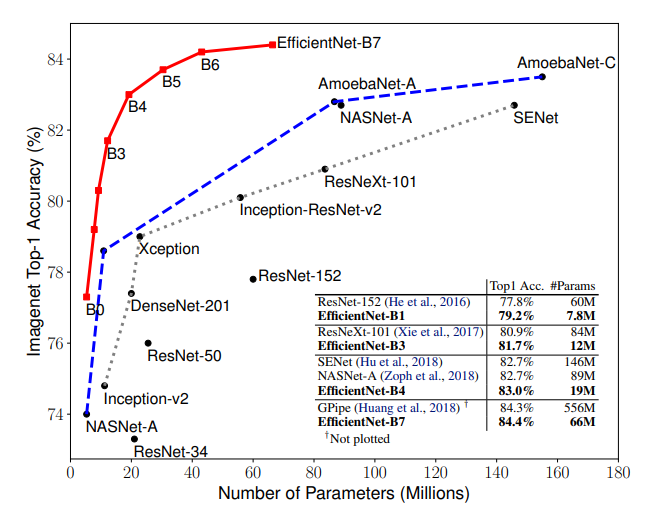
\includegraphics[width=0.7\linewidth]{pictures/ComparisonofEfficient.png}
    \caption{Comparison of EfficientNet with Different Networks on ImageNet\cite{219}}
    \label{fig:ComparisonofEfficient}
\end{figure}

To accommodate diverse detection-box sizes in practice, we adopt an intelligent scaling and padding strategy:\\
    (1) Aspect-ratio preserving scaling to avoid distortion;\\
    (2) Center placement on a 128×128 black canvas for uniform input size;\\
    (3) Data augmentation with horizontal flips, random rotations (±15°), color jitter, and random erasing to enhance generalization.\\
This preprocessing aligns training and inference distributions and mitigates domain shift. As shown in \textbf{Fig.}~\ref{fig:OverallFeatureExtraction}, the overall feature extraction and output process in our system is illustrated.
\begin{figure}[H]
    \centering
    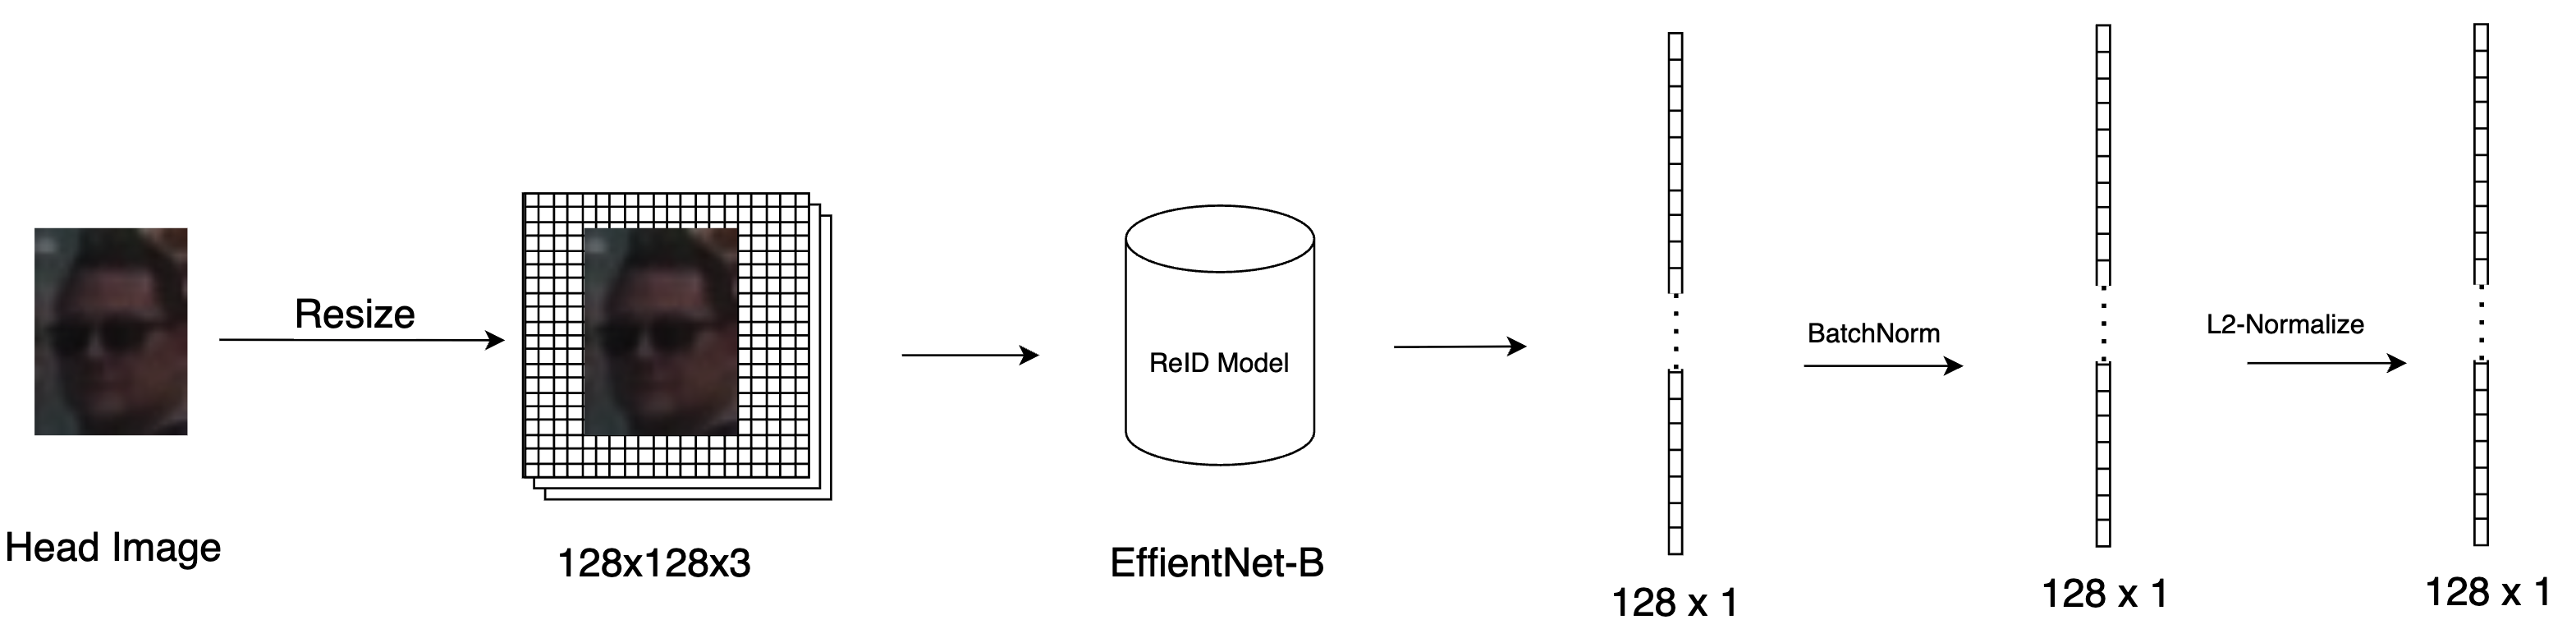
\includegraphics[width=0.9\linewidth]{pictures/OverallFeatureExtraction.png}
    \caption{Overall Feature Extraction and Output in Our System}
    \label{fig:OverallFeatureExtraction}
\end{figure}

For ReID, we use the triplet loss:
\begin{equation}
L_{triplet} = \max(0, d(a,p) - d(a,n) + \alpha)
\end{equation}
with $\alpha=0.5$. Training uses AdamW (lr=2×10⁻⁴, weight decay=1×10⁻⁴), OneCycleLR scheduling, mixed precision, and batch size 32.

\subsubsection{Data Association}
Data association matches detections to tracks by combining motion and appearance cues. The similarity measures include:\\
• Mahalanobis distance for motion compatibility: $D_M(i, j) = (d_j - y_i)^T S_i^{-1} (d_j - y_i)$, where $d_j$ is the detection, $y_i$ the prediction, and $S_i$ the covariance \cite{105}.\\
• Cosine distance for appearance: $D_C(i, j) = \min \{ 1 - \mathbf{r}_j^T \mathbf{r}_k^{(i)} \mid \mathbf{r}_k^{(i)} \in R_i \}$, where $R_i$ stores up to 100 recent descriptors per track \cite{105}.\\
• Combined cost: $c_{i,j} = \lambda D_M(i,j) + (1-\lambda) D_C(i,j)$ \cite{105}.\\
•Matching strategy:\\
(1)Cascaded matching prioritizes recently seen, longer-lived tracks to reduce ID switches under long occlusions \cite{134}.\\
(2) IoU matching as a fallback for remaining unmatched pairs.\\
(3) Hungarian algorithm solves the final assignment on the combined cost matrix \cite{103}.
\subsubsection{Track Management}
• Initialization: new detections start as "unconfirmed." After two consecutive matches, a track becomes confirmed.\\  
• Termination: tracks unmatched for a prolonged period (e.g., beyond max\_age) are removed.\\
• ID retention and re-identification: combined motion and appearance cues enable re-identification after temporary disappearance; prolonged absence may result in a new ID.

\subsection{Adaptivity Across Scenarios}
Parameters of Kalman filtering (state model, Q, R), gating thresholds, cost weighting, cascade/IoU matching, track lifecycle (n\_init, max\_age), and ReID strength should be tuned to scene characteristics (e.g., irregular motion, noisy detections, frequent occlusion, similar appearances) to maintain robustness.

\subsection{Counting Method}
In our method, given YOLOv11 detections and DeepSORT trajectories, we design a reliable counting algorithm that avoids double-counting. Pure detection summation over frames would overcount the same target repeatedly; counting must therefore operate on unique track IDs.

\subsubsection{Traditional line-crossing and limitations}
The mainstream approach is line/zone crossing \cite{22_hsu_passenger_2020, 204, 68_zhao_detection_2022}, which triggers a count when a trajectory crosses a virtual line. In crowded scenes, brief occlusions near the line can cause severe undercounting (e.g., three people cross abreast but the middle person is fully occluded). As shown in our ablations (\textbf{Chapter} 5), a zero-width line (bandwidth 0) can yield MAPE as high as 93.43%.

\subsubsection{Virtual counting band (ours)}
We propose a Virtual Counting Band with nonzero width near the left/right image borders (\textbf{Fig.}~\ref{fig:VirtualCountingZone}), defined by start/end boundaries as proportions of image width. A target is counted only if it is continuously observed within the band for a preset number of frames. This design:
\begin{itemize}
    \item \textbf{Improves robustness}: a buffer region tolerates brief occlusions and detection jitter;
    \item \textbf{Stabilizes counting}: avoids repeated or spurious counts due to oscillations around a thin line.
\end{itemize}

\begin{figure}[H]
    \centering
    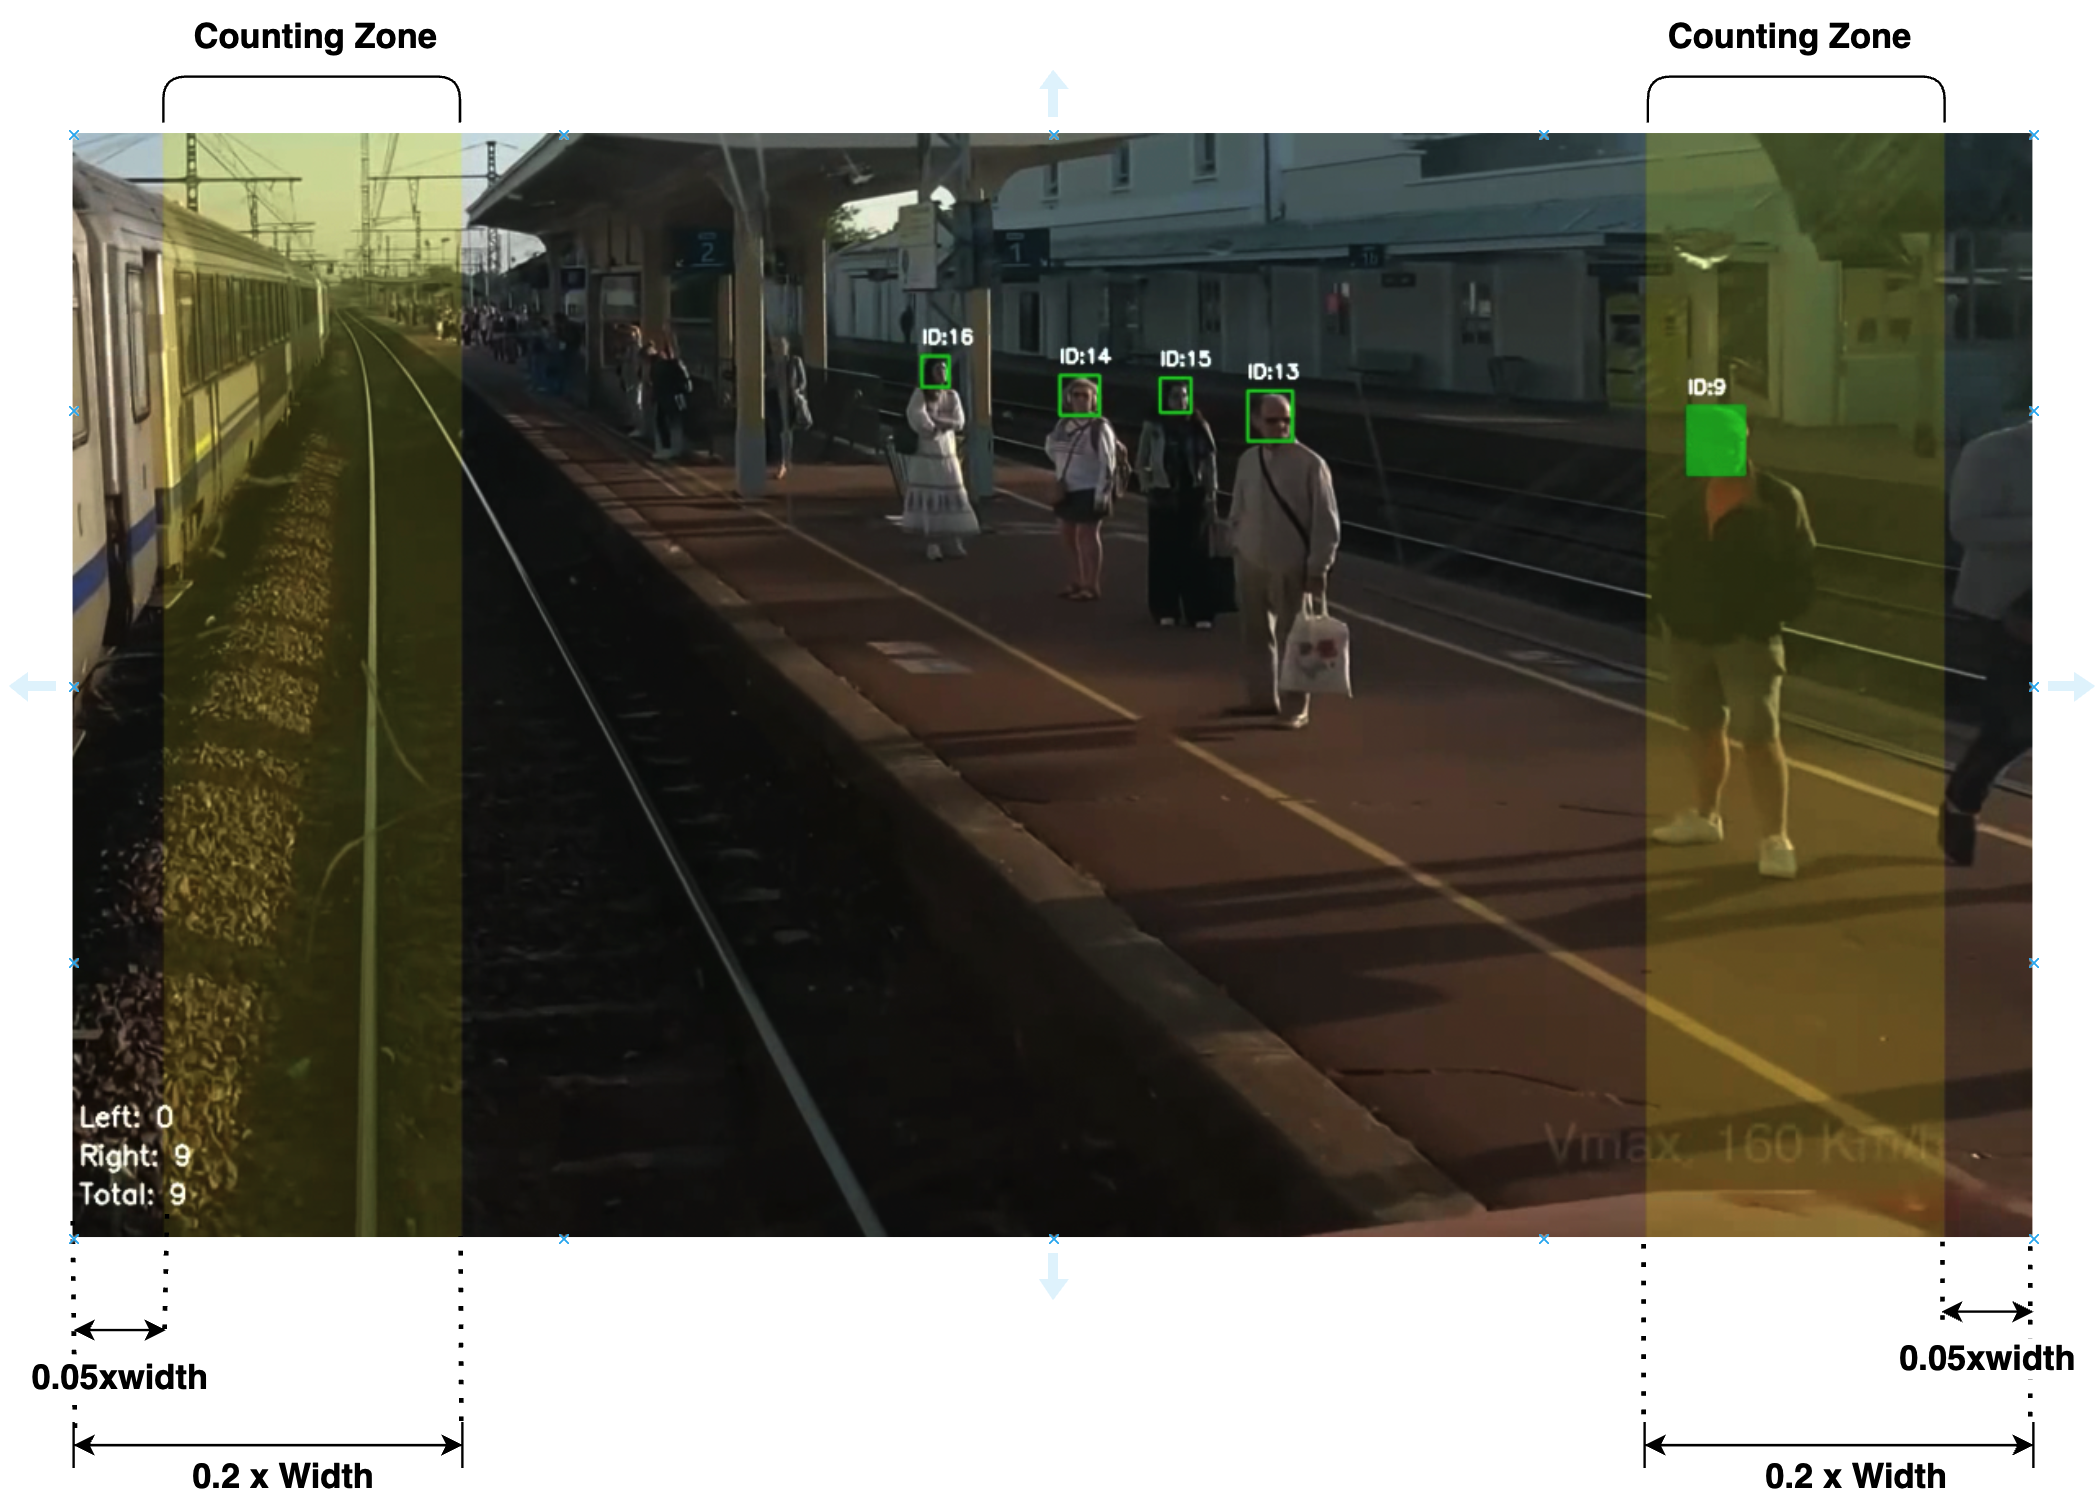
\includegraphics[width=0.7\textwidth]{pictures/VirtualCountingZone.png}
    \caption{Virtual Counting Band Illustration}
    \label{fig:VirtualCountingZone}
\end{figure}
In practice, we set the band to 5\%–20\% of the width from the image borders (relative coordinates for resolution invariance). We maintain per-track state (consecutive in-band frames, counted flag). The target position is the box center; boxes partially outside the frame are clipped for display while preserving original coordinates for logic.

\textbf{Algorithm Implementation:}
\begin{enumerate}
    \item \textbf{Track State Management:} For each confirmed track, maintain state variables: consecutive\_in\_band\_frames, counted\_flag, and side\_assignment (left/right).
    \item \textbf{Band Membership Test:} Compute bounding box center $(u,v)$ and test if $u \in [\text{Start} \cdot W, \text{End} \cdot W]$ for left band or $u \in [W - \text{End} \cdot W, W - \text{Start} \cdot W]$ for right band.
    \item \textbf{Persistence Logic:} If track is in band, increment consecutive\_in\_band\_frames; otherwise reset to 0. When consecutive\_in\_band\_frames $\geq N$ (default N=2) and counted\_flag=False, set counted\_flag=True and increment corresponding side counter.
    \item \textbf{Deduplication:} Maintain global set of counted\_IDs to prevent double-counting across frames.
    \item \textbf{End-of-Video Compensation:} For tracks with consecutive\_in\_band\_frames $> 0$ but $< N$ at video end, apply compensation rule: if consecutive\_in\_band\_frames $\geq N/2$, count the track.
    \item \textbf{Final Aggregation:} Report left count, right count, and final count = max(left\_count, right\_count) to avoid non-platform bias.
\end{enumerate}

Integrity mechanisms include: \\
(1) end-of-video compensation to include targets that nearly meet the persistence threshold; 
(2) deduplication by maintaining the set of counted IDs;\\
(3) using the maximum of left/right counts as the final result (we count one side), which avoids bias from non-platform-side flows.



\subsection{Assumptions and Limitations}
Our formulation assumes: (i) a forward-looking camera with intrinsics $(f,c_x,c_y)$ estimated from representative frames; (ii) average head height $H$ suitable for platform pedestrians; (iii) along-track deceleration during arrivals consistent with the kinematic model. Performance may degrade under extreme lighting or ultra-dense scenes that increase appearance ambiguity or violate motion smoothness. These assumptions are reflected in the calibration and evaluation reported in Chapter~5.

\subsection{Evaluation Metrics}

\subsubsection{Detection Metrics}
We report head detection performance on a static validation set using mAP@0.5 and Recall \cite{74_yolo11_Jocher_Ultralytics_YOLO_2023}. Formally:\\
\textbf{mAP50}: mean AP at IoU threshold 0.5,\\
\begin{equation}
\text{mAP50} = \frac{1}{N}\sum_{i=1}^{N}\text{AP}_i \quad \text{at IoU threshold of 0.5}
\end{equation}
\textbf{mAP50-95}: mean AP averaged over IoU thresholds from 0.5 to 0.95 in steps of 0.05,\\
\begin{equation}
\text{mAP50-95} = \frac{1}{10}\sum_{t=0.5}^{0.95}\text{mAP}_t
\end{equation}
\textbf{Box Precision} and \textbf{Recall} are\\
\begin{equation}
\text{Precision} = \frac{TP_{\text{box}}}{TP_{\text{box}} + FP_{\text{box}}}, \quad
\text{Recall} = \frac{TP_{\text{box}}}{TP_{\text{box}} + FN_{\text{box}}}.
\end{equation}

\subsubsection{Tracking Metrics}
On MOT-RPCH we adopt MOTChallenge metrics: IDF1, MOTA, IDSW, Mostly Tracked(MT), Partially Tracked(PT), Mostly Lost(ML). Following CLEAR-MOT and ID-based protocols (\texttt{py-motmetrics \cite{py-motmetrics} }):\\
\paragraph{CLEAR-MOT}
\begin{align}
\text{MOTA} &= 1 - \frac{\sum_t (FN_t + FP_t + IDSW_t)}{\sum_t GT_t}, \\
\text{MOTP} &= \frac{\sum_{i,t} d_{i,t}}{\sum_t TP_t},
\end{align}
where $GT_t$ is the number of ground-truth objects at time $t$, and $d_{i,t}$ is the distance between a matched hypothesis and ground truth.
\paragraph{Identity-based}
\begin{align}
\text{ID Precision (IDP)} &= \frac{IDTP}{IDTP + IDFP}, \\
\text{ID Recall (IDR)} &= \frac{IDTP}{IDTP + IDFN}, \\
\text{IDF1} &= \frac{2 \cdot IDTP}{2 \cdot IDTP + IDFP + IDFN}.
\end{align}
Additional measures: $IDSW$, Matches, $FP$, $FN$, FAF $= \frac{\sum_t FP_t}{\text{\#frames}}$, and standard Precision/Recall. Track quality: Mostly Tracked (MT, $\geq$80\%), Partially Tracked (PT, 20\%--80\%), Mostly Lost (ML, $<$20\%).

\subsubsection{Counting Metrics}
For $N$ test videos with predicted unique count $\hat{C}_i$ and ground truth $C_i$:
\begin{align}
\text{MAE} &= \frac{1}{N} \sum_{i=1}^{N} | \hat{C}_i - C_i |, \\
\text{RMSE} &= \sqrt{\frac{1}{N} \sum_{i=1}^{N} (\hat{C}_i - C_i)^2}, \\
\text{MAPE} &= \frac{100\%}{N} \sum_{i=1}^{N} \frac{|\hat{C}_i - C_i|}{C_i}, \\
\text{ME} &= \frac{1}{N} \sum_{i=1}^{N} (\hat{C}_i - C_i).
\end{align}



\paragraph{Mean Absolute Error (MAE)} MAE quantifies the average magnitude of the discrepancy between predicted counts and their ground-truth counterparts. Computed as the arithmetic mean of absolute deviations across all samples, MAE offers two key advantages: (i) interpretability—its value directly reflects the mean absolute deviation of estimates from true counts; and (ii) robustness—by imposing a linear penalty on each residual, MAE remains insensitive to outliers and thus delivers a stable summary of overall model performance.

\paragraph{Root Mean Squared Error (RMSE)} RMSE is a widely adopted metric for assessing prediction accuracy. In contrast to MAE, RMSE squares the residuals before averaging and subsequent square-rooting. This quadratic penalty disproportionately amplifies large errors, making RMSE markedly more sensitive to extreme deviations. Consequently, RMSE is the metric of choice when large mispredictions incur disproportionately high costs or when model behavior under adverse conditions must be critically evaluated. By construction, RMSE ≥ MAE; the divergence between the two statistics exposes the presence of occasional large-scale prediction failures.

\paragraph{Mean Absolute Percentage Error (MAPE)} MAPE measures relative, rather than absolute, prediction error. For each sample, the absolute error is normalized by the ground-truth count and expressed as a percentage; MAPE is the average of these percentage errors. Being scale-free, MAPE enables equitable comparison across datasets with disparate count ranges and is particularly informative when performance must remain consistent across both sparse and dense regions. A caveat arises when the true count $C_i$ approaches zero, causing the percentage to explode and rendering MAPE unstable or undefined.

\paragraph{Mean Error (ME), interchangeably termed Bias} ME, interchangeably termed Bias, captures systematic deviation of predictions. It is defined as the average signed difference between estimated and true counts. A positive ME indicates a persistent over-counting tendency, whereas a negative ME signals chronic under-counting. Unlike MAE and RMSE, which quantify error magnitudes, ME diagnoses directional drift and is indispensable for calibrating models to eliminate systematic offsets in safety-critical or metrologically sensitive applications.

